\documentclass[a4paper, dvipdfmx]{jsarticle}

%% Language and font encodings
\usepackage[english]{babel}
%\usepackage[utf8x]{inputenc}
%\usepackage[T1]{fontenc}

%% Sets page size and margins
\usepackage[a4paper,top=3cm,bottom=2cm,left=3cm,right=3cm,marginparwidth=1.75cm]{geometry}

%% Useful packages
\usepackage{amsmath}
\usepackage{graphicx}
\usepackage[colorinlistoftodos]{todonotes}
\usepackage[colorlinks=true, allcolors=blue]{hyperref}
\usepackage{braket, comment, float, listings}

\def\shatai#1{\makebox[2.25zw][l]{\vphantom{#1}\rotatebox{-48.8}{\scalebox{0.875}[1.143]{\rotatebox{41.2}{\smash{\rlap{#1}}}}}}}
\addto\captionsenglish{\renewcommand{\figurename}{図}}

\makeatletter
\def\thanks#1{%
   \footnotemark
   \edef\@tempa{\noexpand\noexpand\noexpand\footnotetext[\the\c@footnote]}%
   \toks@\expandafter{\@thanks}%
   \toks\tw@{{#1}}
   \xdef\@thanks{\the\toks@\@tempa\the\toks\tw@}}
\makeatother

\title{Byteball:価値の蓄積と移転のための分散型システム\thanks{翻訳担当者: \\
     \href{https://twitter.com/hirorobyte}{hiroro} (AG3DGXJCRKJIVSHEMZUIW6AMDRFJVYYW), 1-7章, 26-27章 \\
     \href{http://knskito.com/}{knskito} (QVMGJX367QTJD4TLFYGZNKB256CVTQVX), 8-19章 \\
     inoue (PGRO22WAEBADVAON2UUB5J5PRYJYKSBZ), Abstract, 20-25章 \\
     \href{https://twitter.com/yurwo}{ゆりお} (J6AJTK6SWWBKSOFZ7HT4YBVWSG3ZW4ZU), 28-31章 \\
     }
}
\author{Anton Churyumov\\tonych@byteball.org}
\date{}

\begin{document}
\maketitle

\begin{abstract}
Byteballは、通貨、財産権、債権、株式などの移転可能な価値を表すデータを、改ざん不可能な形式で保管出来る分散型システムです。ストレージユニットは、各々が過去のストレージユニットのハッシュを1つ以上含むことによって相互にリンクされており、これによって過去ユニットの承認とユニット間の半順序の確立が共に行われます。ユニット間のリンクの集合はDAG(有向非巡回グラフ)形式を採ります。データベースへの新規ユニット登録を管理及び調整する単一・中央の主体は存在せず、署名と追加データサイズ(バイト単位)に等しい手数料の支払いによって、誰でも新規ユニットを追加することが可能です。手数料は、新たに追加されたユニットのハッシュを後に自身のユニットに含めることで承認したユーザーによって収集されます。新規ユニットが追加されるにつれ、過去の各ユニットは自身のハッシュを含む後続のユニット群によって、直接的または間接的に更に多くの承認を受けることになります。

分散データベースにデータを追加するための支払いには、‘bytes’と呼ばれる内部通貨が用いられます。また、資産や債権、株式などを表す他の通貨(アセット)も誰もが自由に発行出来ます。ユーザーは財/サービスの支払いや通貨の交換のためにbytesやアセットを相互に送ることが出来、価値移転のためのトランザクションはストレージユニットとしてデータベースに追加されます。もし2つのトランザクションが同じoutputの支払いを試みており(二重支払い)、かつそれらの間に半順序が存在しない場合には、両方ともデータベースに受け入れられますが全順序で先に来た方のみが有効となります。全順序はwitness(証人)と呼ばれる知名度のあるユーザー達が署名したユニットによって形成される、DAG上の単一のチェーン(メインチェーン)を選択することで決定されます。メインチェーン上で先にハッシュが含まれているユニットが、全順序においても先にあると見なされます。ユーザーは、全てのストレージユニットの中から信頼出来るwitness達を指名することで、自身にとってのwitnessを選択します。witnessとは実世界のアイデンティティを持つ評価の高いユーザーであり、指名するユーザー達は彼らに二重支払いを決して試みないことを期待しています。witnessの過半数がこの期待通りに行動する限り、全ての二重支払いは直ちに検出され、マークされます。witnessが署名したユニット群はユーザーのユニットの後に積み上げられるため、モデルにはユーザーのユニットの全順序を確定させる決定論的(非確率論的)な基準が存在するのです。

ユーザーは、支払い時に複数の署名が必要となる(マルチシグ)アドレス上に自身の資金を保管することが可能です。また支払いは、他のユーザー(オラクル)によってデータベースへ投稿された特定のデータを検索することで評価される類の条件を含む、他の条件を満たす必要がある場合もあります。

ユーザーは新しいアセットを発行し、その移転可能性を管理するルールを定義することが可能です。ルールには、移転ごとにアセットの発行者が連署しなければならないといった、金融機関が既存の規制を遵守するための1つの手段である支払制限を含めることが出来ます。また、ユーザーは移転記録がデータベースには公開されず、よって第三者からは確認することが出来ないようなアセットを発行することも可能です。この場合、代わりに移転に関する情報がユーザー間で秘密に交換され、データベースにはトランザクションのハッシュ(二重支払い防止用の)支払い証明のみが公開されます。
\end{abstract}

\newpage
\section{序論}
オーウェルの小説『1984年』の中で、主人公のウィンストン・スミスは真理省の記録局で編集者として働いています。そこでは、過去の出来事を、絶えず変化する公式見解に従うように歴史的記録を修正し、失脚してしまった人たちへの言及を削除する作業をしています。すなわち、国家によって殺された上に、歴史や記憶の中からも存在を消されてしまうのです[1]。ここで私達が提案するものは、書き換えが不可能なデータストレージです。これは、分散型の非中央集権的データベースであり、記録を完全に変更することも削除することも出来ません。

Bitcoin[2]は、Bitcoinと呼ばれる電子通貨単位の所有権を追跡するという特定の目的のために設計された、改ざん不可能な最初のシステムでした。Bitcoinでは、通貨の全ての移転は、コインの現在の所有者によってデジタル署名されたトランザクションとして表され、トランザクションはブロックにまとめられ、全てのブロックが1つのチェーン(ブロックチェーン)にリンクされます。ブロックチェーンの安全性は、大規模なコンピューティングリソースに保証されたproof of work(PoW)によって保護されています。従って、ブロックチェーンに刻まれたことを書き換えようとするあらゆる試みは、既に消費されているよりもさらに大きなコンピューティングリソースが必要になります。

Bitcoinが登場した直後に、これは単に相手への信頼が必要のないP2P電子通貨以上のものであることが明白となりました。その技術は、他の問題を解決するための新しいアイデアの源となりました。同時に、Bitcoinの欠点や限界も同様に明確になりました。ByteballはBitcoinをより一般化して、あらゆるデータの改ざんを防止するストレージになるように設計されています。つまり、単なる電子通貨の移転だけでなく、Bitcoinの幅広い普及と成長を阻害する最も重要な欠点を取り除くように設計されています。

\emph{ブロック:}Bitcoinでは、トランザクションはブロックにまとめられ、ブロックは単一のチェーンに連なります。ブロックは一方向に直線状に繋がっているため、時間間隔とブロックサイズはノード間でほぼ同期するように最適化されています。そのため、ノードは新しいブロックを生成するのに必要な時間よりもはるかに高速に新しいブロックを共有出来ます。これにより、全てのノードが最後のブロックと同じブロックを参照する可能性が高くなり、ブロックの分岐が最小限に抑えられます。Bitcoinが成長するにつれて、ブロックはどんどんと扱いにくくなっていきます。それらはサイズが制限されていたり、ネットワークの全てのノードへ伝播するのに時間がかかり過ぎたりします。前者の場合は成長が阻害され、後者の場合はどれが最後のブロックであるかの不確実性が増大し、また後に孤立してしまうチェーンを伸ばすためにコンピューティングリソースが無駄になってしまいます。しかしByteballでは、ブロックは存在せず、各トランザクションがブロックの役割を担い、かつそれらは単一のチェーンに接続する必要がありません。代わりに、トランザクションは複数の以前のトランザクションにリンクされており、トランザクション全体は単一のチェーンではなく、DAG(有向非巡回グラフ)の形式をとっています。DAGベースの設計は最近多くの注目を集めています[3-5]。

\emph{コスト:}Bitcoinのトランザクションは安全です。なぜならトランザクション後に生成されたブロックに含まれる全てのPoWをやり直すのは非常にコストがかかるためです。しかし、これはまた、いかなる攻撃も撃退するのに十分なPoWを構築するためにはコストをかける必要があることを意味します。このコストは、PoWを構築するために必要な電力として費やされます。ここで重要なことは、この資金はBitcoinのエコシステムの外(電力会社など)に支払われるということです。つまり、Bitcoinのコミュニティ全体から外部への資金流出を伴っているということです。Byteballでは、PoWの代わりに、Bitcoinよりもずっと前から知られていた古いアイデアに基づいた別の合意形成アルゴリズムを使用しています。

\emph{ファイナリティ:}Bitcoinにおけるトランザクションの確定は確率論的になされます。トランザクションが覆されることがないと言える厳密かつ単純な基準はありません。むしろ、より多くのブロックが追加されるにつれて、トランザクションが覆される確率が指数関数的に減少するということのみを主張することが出来ます。このコンセプトは数学に精通している人にとっては明白ですが、コインの所有権が白か黒かはっきりしていることを期待している平均的な人にとっては難しいかもしれません。 さらに複雑なことに、トランザクションの確定はその金額にも依存します。金額が少なければ、誰もあなたに二重支払いをしかけようとしないことは当然明白です。しかし、預ける金額がブロック報酬(執筆時点では12.5 BTC)を上回っている場合には、支払人がハッシュパワーを一時的に借りて、あなたを受取人とするトランザクションを含まない別ブロックのチェーンをマイニングするという可能性が考えられるでしょう。従って、トランザクションの価値が高いとそれが十分に最終的であると言えるまでに、より多くの承認を待たなければなりません。Byteballには、トランザクションがどれほど大きくても、いつトランザクションが確定するかについての決定論的な基準があります。

\emph{交換レート:}Bitcoinの価格は変動が激しいことが知られています。より大きな問題は、この価格が変動するだけでなく、何にも紐づけられているわけではないということです。株式やコモディティ価格もかなり変動しますが、その裏にはファンダメンタルズ的な要素が存在します。株価は、主に、会社の売上、収益、負債対資本比率などと関連します。コモディティの価格は、とりわけ、様々なサプライヤーにおける生産コストに依存します。たとえば、原油価格が一部のサプライヤーの生産コストを長期間下回ると、そのサプライヤーの操業は停止し、生産量が減少することで、最終的に価格が上昇することになります。このように、ネガティブフィードバック・ループが機能します。Bitcoinには、そのようなファンダメンタルズはなく、ネガティブフィードバックはありません。\$500というBitcoinの価格は、\$50,000や\$5といった価格以上に正当化されているわけではなく、Bitcoinの価格が現在の位置から動いても、価格を押し戻すような経済的な力が生じるわけではありません。単に無秩序な動きなのです。Byteballでは、Byteballのデータベースにデータを追加するために基本通貨としてbytesが使用されます。1 Kbのデータを追加するために1,000 bytesが支払われます。これは、このデータベース内ストレージの効用を測る尺度となり、実際のユーザーは、これに対して妥当な価格がいくらであるかを検討することになるでしょう。もしbytesの価格があなたのニーズに見合う金額を超えた場合、bytesの保有量を減らそうとするでしょう。そのため、必要なbytesの購入量は減少し、需要も減少し、その結果価格は下落します。これは、必要性が需要を決める全ての財/サービスに共通したネガティブフィードバックであり、投機ではありません。bytesでの支払いに加えて、他のアセットを発行して支払い手段として使用することも出来ます。これらのアセットは、例えば、フィアット通貨または自然単位(kWhまたは石油のバレルなど)で表された債務を示すこともありえるでしょう。そのようなアセットの価格は、紐づいている通貨やコモディティに自然と結びつきます。

\emph{プライバシー:}全てのBitcoinのトランザクションとアドレス残高は、ブロックチェーン上で可視化されています。取引や残高を不明瞭にする方法はありますが、それは人々が通貨に期待しているものではありません。Byteball上でのbytes(基本通貨)のトランザクションは同様に可視化されていますが、追跡することが非常に困難なもう1つの通貨(blackbytes)があります。

\emph{コンプライアンス:}Bitcoinは、所有者が自身のお金を完全にコントロールすることが出来る匿名通貨として設計されました。その目標は達成されました。しかしそれがゆえに、Bitcoinは既存の規制とはなじまないものであり、金融業界で使用するには不適切なものになっています。Byteballでは、Bitcoinのように全く制限が無い場合から、全ての移動に発行者(例えば銀行)の連署を必要とする場合や、ホワイトリスト内の限られたユーザー間にのみ転送を制限するような場合まで、譲渡可能性に関してあらゆるルールを持つアセットを発行することが出来ます。

\section{データベース構造}

ユーザーは、データベースにデータを追加したい時に、新しいストレージユニットを作成し、それをピア達に伝播させます。ストレージユニットには、(とりわけ)以下を含みます:
\begin{itemize}
    \item 保存するデータ。1つのユニットには、\emph{メッセージ}と呼ばれる複数のデータパッケージを含めることが出来ます。 メッセージにはさまざまな種類があり、それぞれに独自の構造があります。メッセージタイプの1つは\emph{送金}で、これはbytesまたは他のアセットをピアに送信するために使用されます。
    \item ユニットを作成した1人以上のユーザーの署名。ユーザーは各自のアドレスで識別されます。個々のユーザーは、Bitcoinのように複数のアドレスを持つことが出来ます(推奨)。最も単純なケースでは、アドレスはBitcoinと同様に公開鍵に由来しています。
    \item ハッシュで識別された1つ以上前のユニット(親ユニット)への参照。
\end{itemize}
親への参照は、ユニットの順序(これまでの半順序のみ)を確立し、ブロックチェーン構造を一般化しています。連続するブロック間の親と子の関係は1対1に限定されているわけではないので、苦労してほぼ完全に同期させる必要はなく、また大きいレイテンシや高スループットも安全に対応出来ます:1つのユニットあたりの多くの親や子が存在することになるだけです。親-子のリンクを遡ると、同じユニットが複数の後続するユニットに参照されている分岐や、同じユニットが複数の先行するユニットを参照している統合を、多く確認することが出来ます(開発者はこれらの分岐や統合を既にgit上で見慣れているでしょう)。この構造は、有向非循環グラフ(DAG)として知られています。ユニットは頂点となり、親-子のリンクはグラフの辺を形成するのです。

\begin{figure}[htbp]
  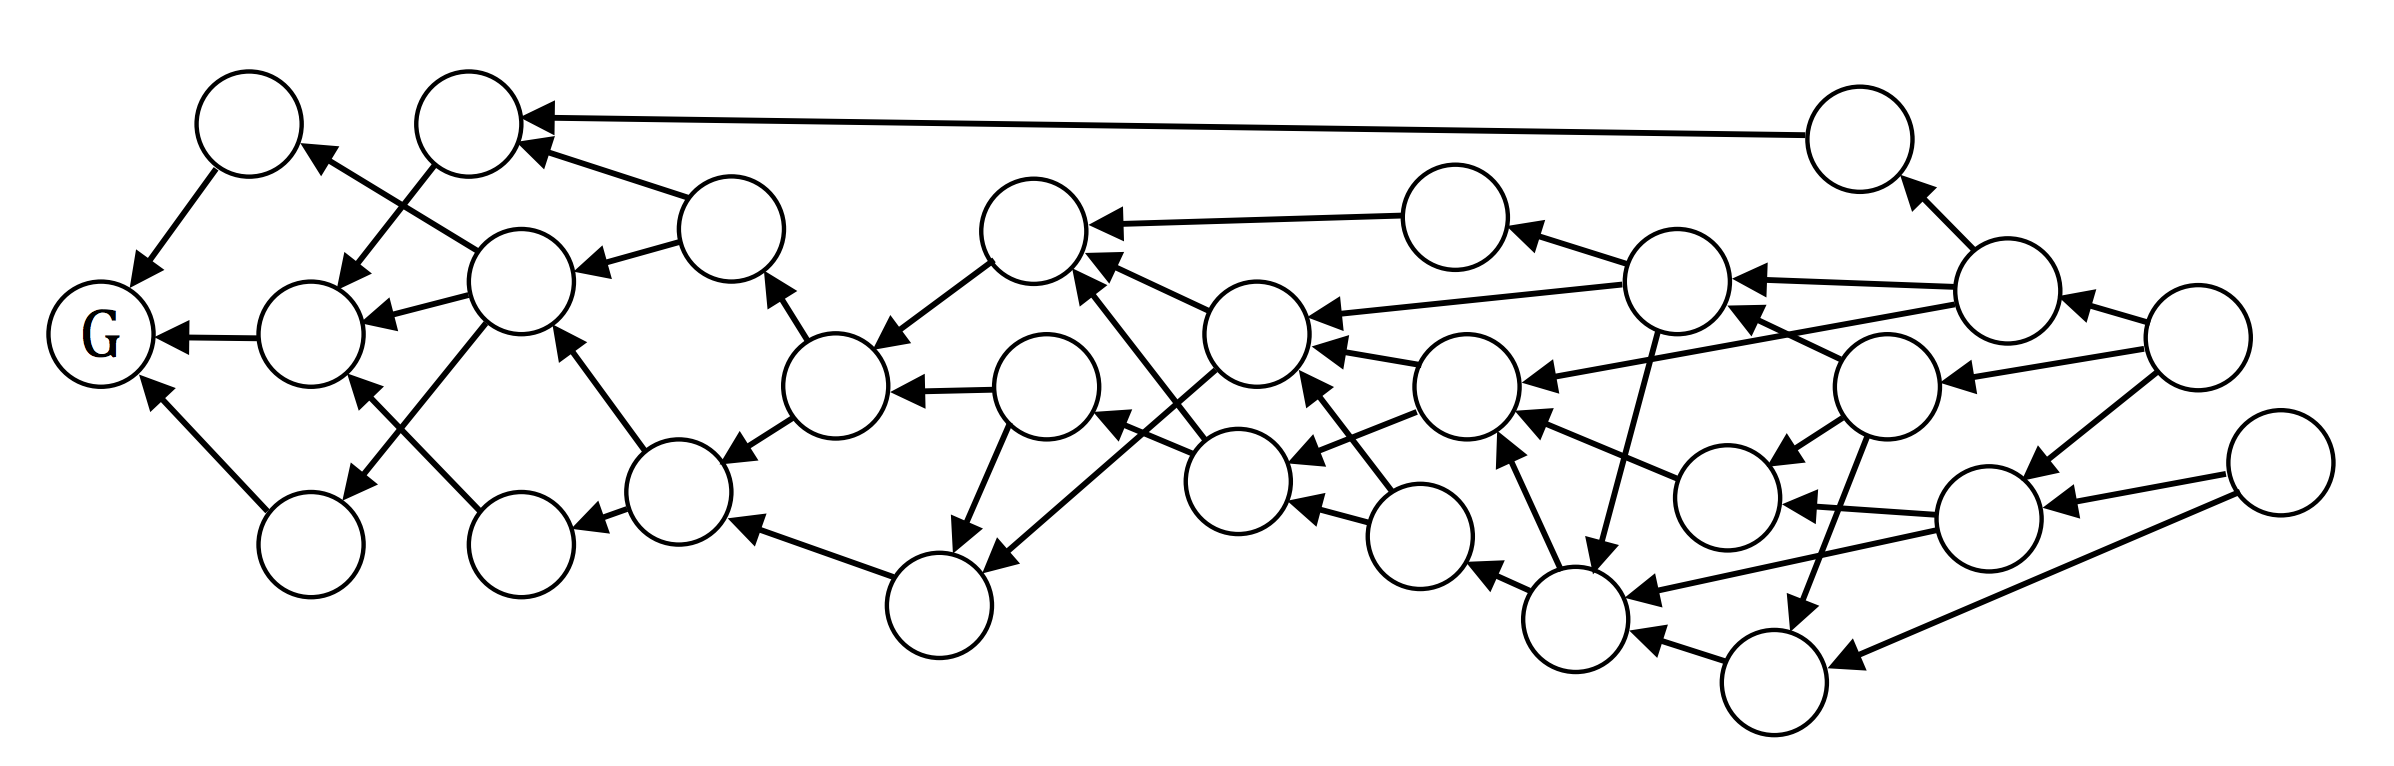
\includegraphics[width=\linewidth]{fig1.png}
  \caption{DAGで接続されるストレージユニット。矢印は子から親を指し、Gはジェネシスユニットを示す。}
\end{figure}

新しいユニットがめったに届かない特殊なケースでは、DAGは、時折分岐しては素早く統合するような状態となり、ほとんどチェーンのように振る舞うでしょう。

新しいブロックが以前の全ブロック(及びそこに含まれるトランザクション)を承認するブロックチェーンの場合と同様に、DAG内の全ての新しい子ユニットは、自身の親、全ての親の親、親の親の親、・・・、を承認します。ユニットの編集を試みる場合には、ハッシュも変更せねばなりません。子ユニットの署名とハッシュの両方が親ハッシュによって変わるため、このような改ざんは必然的に、編集対象のユニットを参照する全ての子ユニットを成り立たなくしてしまいます。従って、全ての子ユニットと協調するか彼らの秘密鍵を盗み出すかをしなければ、ユニットを改ざんすることは不可能です。そして、子ユニットも、自身にとっての子ユニット達(元のユニットの孫ユニット)との協調がなければ改ざんすることは出来ません。あるユニットがネットワークに伝播され、他のユーザがそのユニットの上に別のユニットを構築する(親として参照する)ようになると、このユニットを改ざんするのに必要な二次的な修正の数は雪だるま式に増加します。これが私達がこのデザインをByteballと呼ぶ理由です(雪の一片がデータのbytesに相当します)。

ブロックの発行がまれであったり特権階級のユーザだけがブロックを承認するようなブロックチェーンとは異なり、新しいByteballのユニットではユニット生成直後から承認が蓄積し始め、その承認は別の新たなユニットが生成される度に誰もが行えます。そこには通常のユーザーとマイナーといった2階層のシステムはありません。代わりに、新しいユニットを追加する際にその署名者が以前の全ユニットを承認することによって、ユーザーはお互いに助け合うのです。

過去の取引を改ざんしようとするために大きな計算量を必要とするBitcoinとは異なり、Byteballにおいて過去の記録の改ざんには、多くの、そして増加し続ける他のユーザーとの協力が必要となり、しかもそのほとんどは匿名の他者です。従って過去の記録の改ざん耐性は、接触が困難で協力することに関心がなく、かつ一人ひとりが改訂に対して拒否権を持つ過半数の人達との調整が必要であるという複雑性に基づいています。

親ユニットを承認することで、そのユニットには親の情報が含まれることになります。親の完全な内容が含まれるわけではなく、親のハッシュの情報を組み込むことになります。同じように、ユニットは間接的に親の親などの情報を含むため、全てのユニットは結局はジェネシスユニットを含むことにつながっているのです。

ユニットには冗長な親を参照することが出来ないというプロトコルルールがあります。それは、承認する複数の親が子と親の関係になっているような場合です。例えば、ユニットBがユニットAを参照する場合、ユニットCはユニットAとユニットBの両方を同時に参照することは出来ません。Aは既にBのユニット内に組み込まれています。このルールは、DAGにとって有用でない不要なリンクを取り除くために存在するのです。

\section{ネイティブ通貨:bytes}
次に、無意味なメッセージによるスパム攻撃からデータベースを守るための抵抗を導入します。スパム対策用の参入障壁は、ユーザーにとってのストレージの効用とネットワークにとってのストレージの費用とを大まかに反映するべきでしょう。これら両方の最も単純な尺度は、ストレージユニットのサイズです。従って、グローバルな分散データベースにデータを格納するには、\emph{bytes}と呼ばれる内部通貨で手数料を支払う必要があります。支払う金額は、保存するデータのサイズ(全てのヘッダーや署名などを含む)に等しくなります。最初に導入された際は銀1ポンドと等しかったイギリスのスターリング・ポンドと同様、通貨の名前はその価値を反映しているのです。

ネットワーク全体の利益に見合ったインセンティブを保つために、データサイズの計算ルールには例外を1つ設けています。それは、ユニットのサイズを計算する時に、実際の数に関わらず必ず2つの親を持つとする仮定です。従って、親ユニットの2つのハッシュ分のサイズが常にユニットサイズに含まれることになります。この例外によって、ユーザーはコストを最小限に抑えるために1つの親しか含まないといった試みを行わなくなるでしょう。どれだけ多くの親が含まれていても、この費用は同じものとして計算されます。

DAGを可能な限り小さく保つために、ユニットを最初に親として含めたユーザーにそのユニット手数料の一部を支払うことによって、ユーザーに可能な限り多く、そして可能な限り新しい親を含める(前述の通り、これは手数料の大きさに悪影響を及ぼしません)インセンティブを与えます。この「最初」については、後に正確に定義します。

bytesは、ストレージ手数料の支払いのためだけでなく、商品やサービスの支払いや、他のアセットとの交換のために使うことが出来ます。送金するために、ユーザーは次のような送金メッセージを含む新しいユニットを作成します(ここからはJSONを使用してデータ構造を記述します)。

\begin{lstlisting}[basicstyle=\ttfamily\footnotesize, frame=none]
{
    inputs: [
        {
            unit: "hash of input unit",
            message_index: 2, // index of message where this utxo was created
            output_index: 0 // index of output where this utxo was created
        },
    ...
    ],
    outputs: [
        {
            address: "RECEIVER ADDRESS",
            amount: 15000 // in bytes
        },
    ...
    ]
}
\end{lstlisting}

\noindent メッセージには以下が含まれます:
\begin{itemize}
    \item outputsの配列:bytesを受信する1つ以上のアドレスと、アドレスが受け取るbytesの量。
    \item inputsの配列:送金額の資金として使用される、以前のoutputsへの1つ以上の参照。これらは、過去に署名者のアドレス宛に送られた、まだ使用されていないoutputsです。
\end{itemize}

\noindent inputの合計値は、outputと手数料の合計値と等しくなければなりません(input量は以前のoutputから読み込まれ、支払い時には明示されません)。また、ユニットは署名者の秘密鍵によって署名されます。

流通中の総bytes数は$10^{15}$であり、この数は一定に保たれます。 全bytesはジェネシスユニットで発行され、ユーザーからユーザーに移転されます。また、手数料はネットワークの健全性を維持するのに貢献している他のユーザー達(後に詳述)によって収集されるため、流通し続けます。$10^{15}$という数字は、JavaScriptで扱える最大の整数を採用しており。金額は整数のみ使用可能です。より大きな通貨単位は、1,000 bytesを1 kilobyte(Kb)、100万bytesを1 megabyte(Mb)など標準的な接頭語を用いることで表現することが出来ます。

\section{二重支払い}
ユーザーが同じoutputを2回使用しようとすると、次の2つの状況が発生する可能性があります:

\begin{enumerate}
    \item 同じoutputの使用を試みる2つのユニット間に半順序が存在する、すなわち、一方のユニットにもう一方のユニットが(直接的または間接的に)含まれている場合。この時には、明らかに順番が後のユニットを安全に拒否すべきでしょう。
    \item ユニット間に半順序が存在しない場合。この場合には、両方が承認されます。ただし、これらのユニットは新しいユニットの下に十分深く埋め込まれると、全順序が確立されます(その仕組ついては以下を参照して下さい)。全順序において先に現れるユニットが有効とみなされ、他方は無効とみなされます。
\end{enumerate}

全順序の定義を単純化するために、もう1つのプロトコルルールがあります。同じアドレスが複数のユニットを投稿する場合、全ての後続ユニットは以前の全ユニットを(直接的または間接的に)含めなければなりません。つまり、同じアドレスからの連続したユニットは半順序を確立する必要があります。言い換えれば、同じ署名者による全てのユニットには順番が付いていなければならないのです。

もし誰かがこのルールを破り、半順序が確立されていないユニット(順番未決定ユニット)を2つ投稿した場合、例え同じoutputでの送金を試みていなくとも、それらは二重支払い扱いとなります。そのような順番未決定ユニットは、上記の状況2で説明したように処理されます。

\begin{figure}[htbp]
  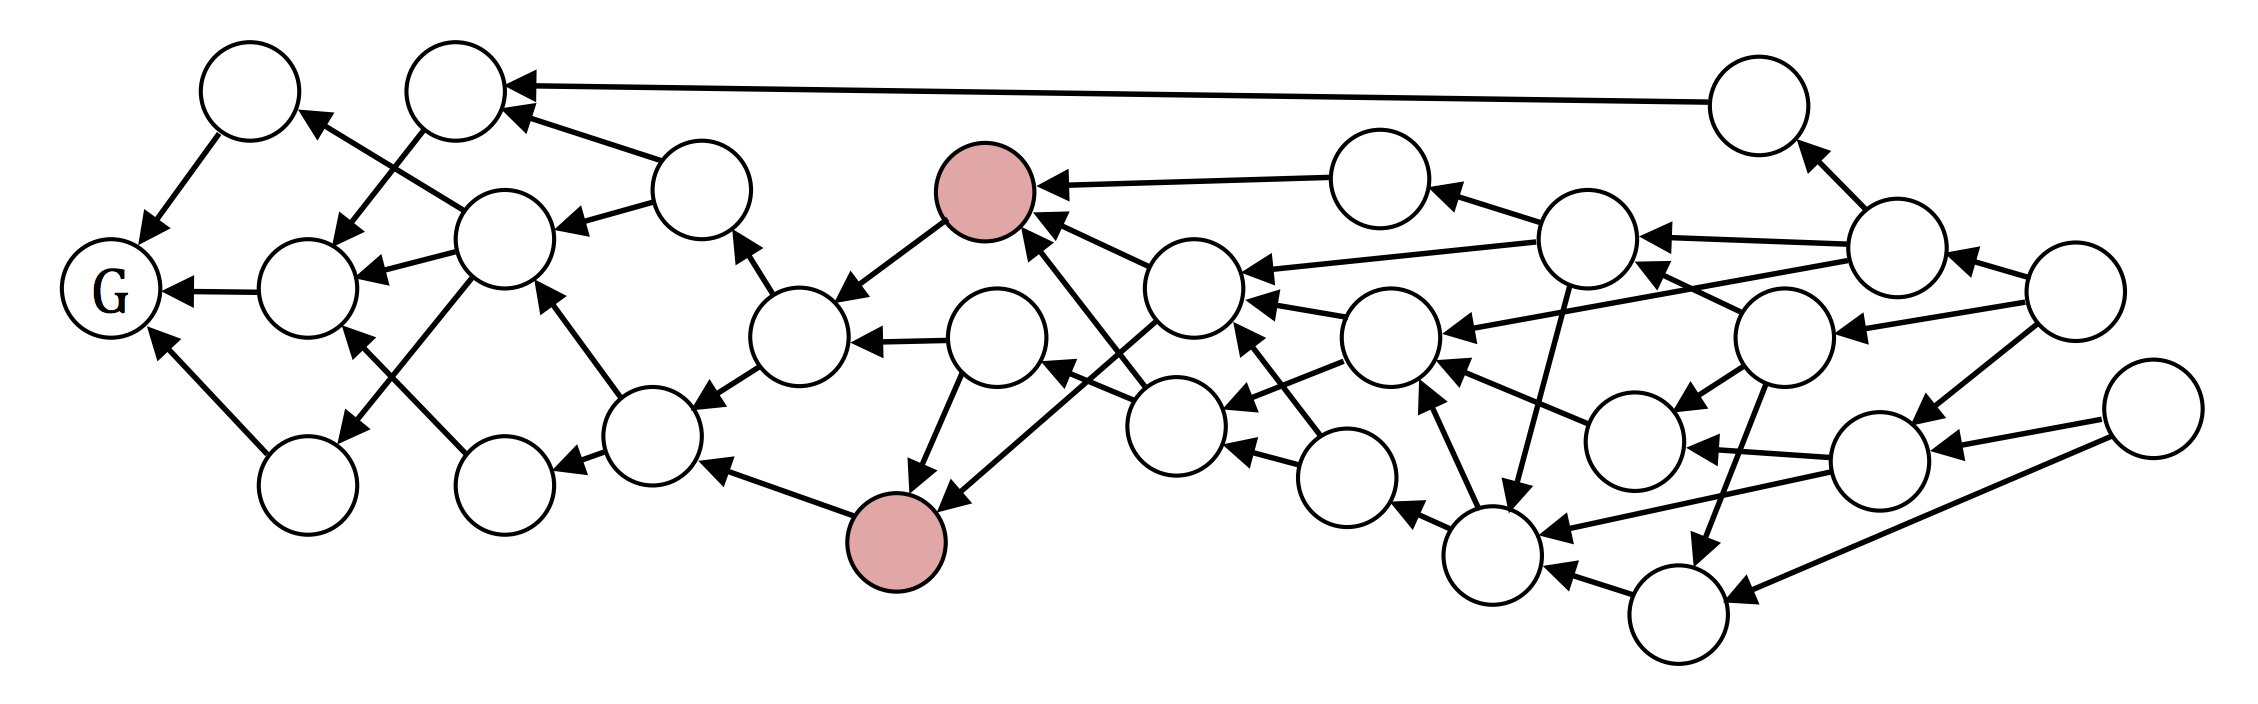
\includegraphics[width=\linewidth]{fig2.png}
  \caption{二重支払いユニット間に順序がない例。}
\end{figure}

ユーザーがこのルールに従いながらも同じoutputの使用を2回試みた場合、その二重支払いは明確に順序付けされ、上記の状況1に則して後のユニットを安全に拒否することが可能です。よって、順番未決定では無い二重支払いについては容易に除外されます。

このルールは実際、非常に自然なものです。ユーザーが新しいユニットを作成する時、彼は直近の他のユニットを自分のユニットの親として選択します。それらを親のリストへ入れることにより、これらのユニットを既に確認したということを宣言します。つまり彼は、親の親、親の親の親...とジェネシスユニットに至るまでの全ユニットを確認したことになるのです。この巨大な集合には、当然彼自身が作成したものも含まれ、それらも確認済みとなります。

あるユニットを(親を介して間接的にでさえ)含まない場合、ユーザーは自分がそれを見たことを否定することになります。もしユーザーが自分が以前作成したユニットを含めずに、その確認を否定した場合、それは奇妙であり何か怪しいことが起こっていると言えるでしょう。私達ははそのような行動を阻止します。

\section{メインチェーン}
私達のDAGは特別なDAGです。通常利用する際には、新しいユニットをごく直近のユニットにリンクするため、DAGは一方向にしか成長しません。内部に多くのワイヤーを結び合わせた太い紐のように描写することが出来ます。この特性は、私達がDAG内の子-親のリンクに従って1つのチェーンを選択し、全てのユニットをこのチェーンに関連付けられることを示しています。全てのユニットは私達がメインチェーンと呼ぶこのチェーン上に直接存在しているか、グラフの端に沿って比較的小さいホップ数で到達可能なところにあります。これは、脇道が接続している高速道路のようなものです。

メインチェーンを構築する1つの方法は、あるユニットが持つ全ての親に対して、その中から1つを「最良の親」として選択するアルゴリズムを構築することです。 選択アルゴリズムは、問題としているユニットに関連して利用可能な情報、すなわち、そのユニット及びそのユニットの全ての祖先に含まれるデータにのみ基づいていなければなりません。DAGの任意の頂点(子を持っていないユニット)からスタートして、最良の親からなるリンクに沿って履歴を遡ります。このように進むことで、私達はメインチェーンを構築し、最終的にはジェネシスユニットに到達します。特定のユニットから開始して構築されたメインチェーンは、新しいユニットが追加されても決して変更されないことに注意して下さい。これは、各ステップにおいて、私達は子から親に移動しており、既存のユニットは決して新しい親を得ることが出来ないからです。

もしも別の頂点から開始したら、別のメインチェーンを構築することになります。ここで注目すべきは、履歴を遡る間にこれら2つのメインチェーンが交叉した場合は、その交点の後は両者が同じ経路を辿るということです。最悪の場合、メインチェーンはジェネシスユニットでのみ交差します。しかし、ユニットを構築するプロセスがユーザー間で調整されていないとすれば、頂点から離れすぎないように収束するメインチェーンの集合を見つけることが出来るでしょう。

\begin{figure}[htbp]
  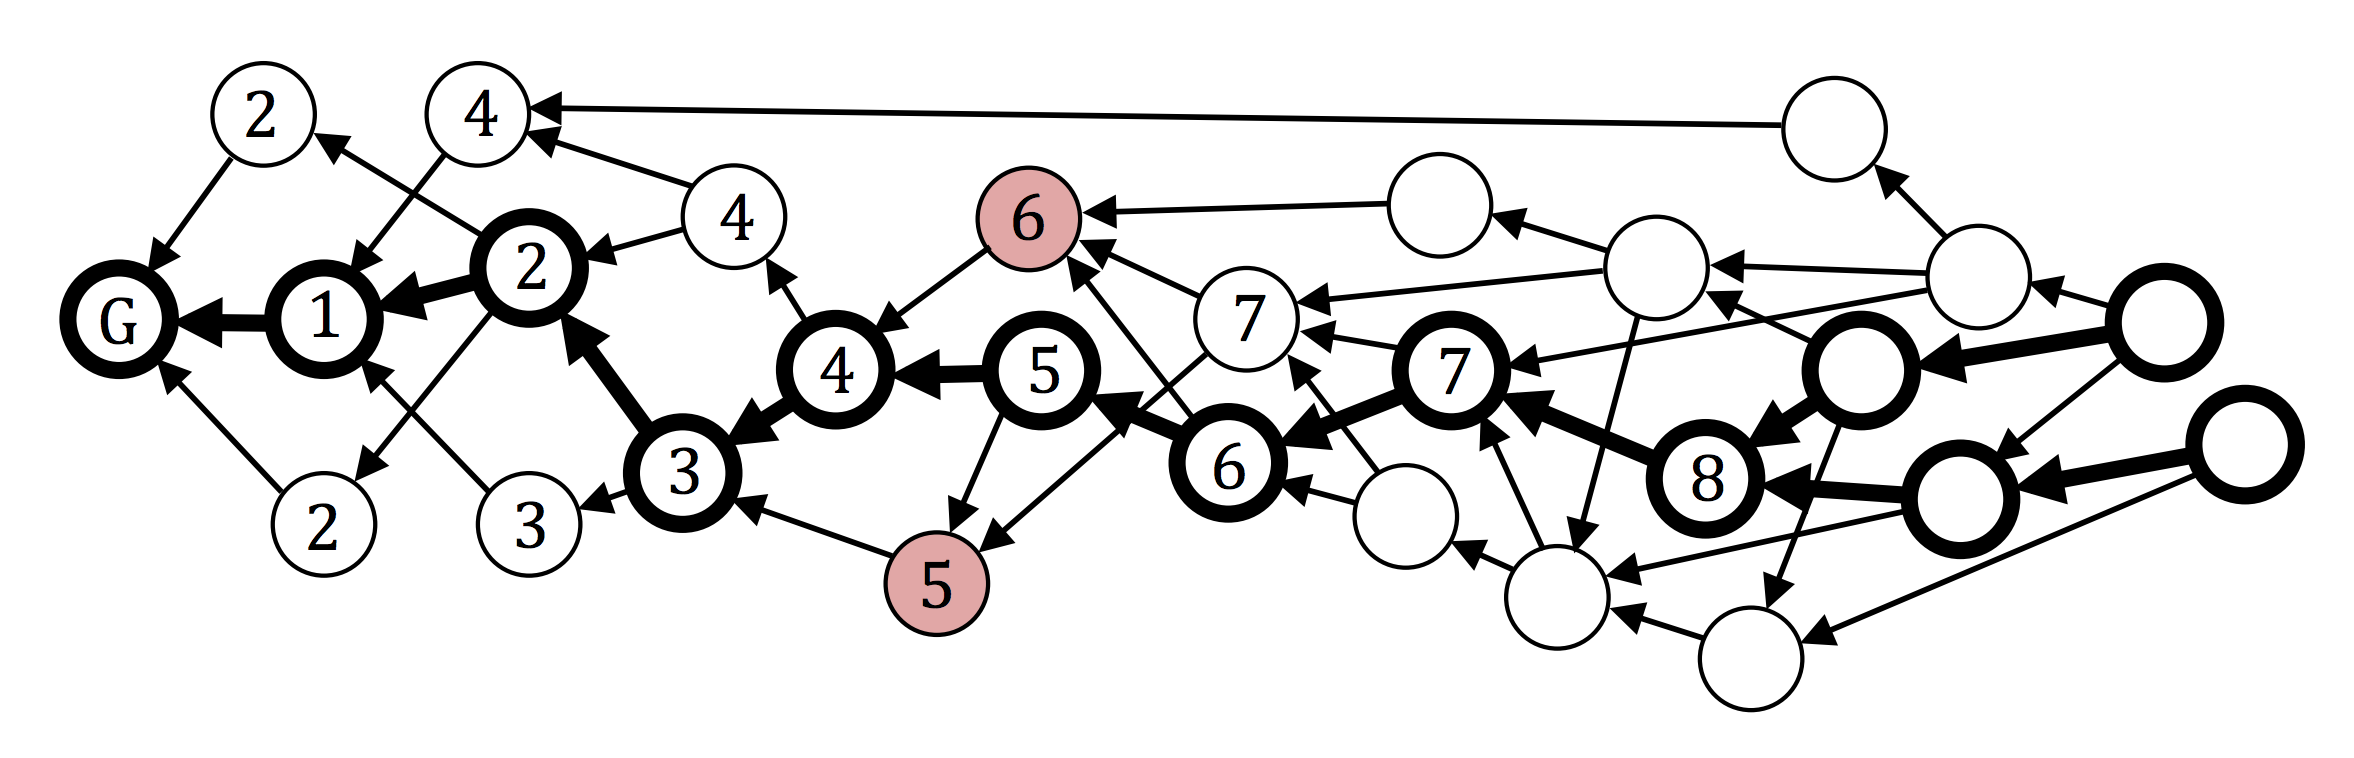
\includegraphics[width=\linewidth]{fig3.png}
  \caption{異なる子が存在しないユニットから構築されたメインチェーンが交差し、そして同じ経路を進む様子。2つの二重支払いのうち、低いメインチェーンインデックス(MCI=5)を持つユニットが承認され、もう片方(MCI=6)は無効とみなされる。}
\end{figure}

一度メインチェーン(MC)を構築すれば、2つの相反する順番未決定ユニット間で全順序を確立することが出来ます。まず最初にメインチェーンに直接存在するユニットにインデックスを付けていきましょう。ジェネシスユニットをインデックス0とし、ジェネシスユニットの子である次のMCユニットはインデックス1、といったように、MCに沿って進みながら、MC上に存在するユニットにインデックスを割り当てます。MC上にないユニットについては、このユニットが最初に(直接的または間接的に)含まれるMCのインデックスを見つけることが出来ます。このようにして、全てのユニットにMCインデックス(MCI)を割り当てることが出来ます。

そして、2つの順番未決定ユニットのうち、MCIが小さいユニットはより早いものであり、有効であるとみなされ、もう一方のユニットは無効であるとみなされます。もしも両方の順番未決定ユニットが同じMCIを持つことが起こった場合、低いハッシュ値(base64エンコーディングで表される)を持つユニットが有効であるというタイブレーカールールがあります。ここでは、最終的には敗れるものを含めて、全てのバージョンの二重支払いを保持する点に注意して下さい。DagCoin [3]は、競合する全てのトランザクションの格納と、どちらのトランザクションを有効として扱うかの決定を示した最初の公開研究でした。

特定のユニットから構築されたMCは、このユニットの署名者が過去の事象の順序をどう考えているか、すなわち過去の履歴に関する彼の視点を示しています。そのため、上記のように、順序はどの順番未決定ユニットが有効とみなされるかを暗示しています。特定のユニットの全ての親の中から最良の親を選択することによって、同時にMCを取捨選択していることに注意して下さい:ユニットのMCは、その最良の親のMCが1つのリンク分だけ前方に拡張されたものになるのです。

多く(または全ての)親ユニットが攻撃者によって作成される可能性があり、また最良の親の選択が本質的には履歴のバーション選択であることを考慮すれば、最良の親の選択アルゴリズムには、子ユニットの視点から「本物」である履歴を選ぶことを求めるべきです。従って、最良とみなすMCを選択するために、私達は全てのMC候補に対してアルゴリズムが実行する「リアリティテスト」を考案する必要があります。

\section{witness}
「リアリティテスト」について考察してみると、ネットワークの参加者の中には、長い間培われた高い評判を持つ匿名ではない人や企業がいたり、ネットワークを健全に保つことに関心のある企業がいることが観測出来るでしょう。私達は以降、彼らのことを\emph{witness}と呼びます。彼らが正直に行動することを期待することは合理的ですが、いかなる単独のwitnessも完全に信頼することは合理的ではありません。もし複数名のwitnessのByteballアドレスを知っており、かつ彼らが十分な頻度で投稿していることが期待される場合、候補となるMCの本物らしさを測るために、そのMCを遡りながらwitness達が署名したユニットの数を数えます(もし同じwitnessが複数回出てきたとしても、一度しか数えません)。過半数のwitnessに遭遇したらすぐに遡ることをやめます。次に、停止した点からジェネシスユニットまでのグラフ上の最長経路の長さを測定します。この長さを、停止したユニットの\emph{レベル}と呼び、そして、テストしているMCを持つ親の\emph{witnessレベル}と呼びます。より大きなwitnessレベルをもたらす候補MCは、より「本物」であるとみなされ、このMCを有する親が最良の親として選択されます。witnessレベルが最大の候補が複数いる場合は、自身のレベルが最も低い親を選択します。引き分けが続く場合は、最小のハッシュ値(base64エンコーディングにおいて)を持つ親を選択します。

このアルゴリズムは、witnessによって署名されたユニットに自然に引き寄せられるようなMCを選択することを可能にし、witnessは本物らしさの代弁者とみなされるのです。例えば、もしも攻撃者がネットワークの信頼出来るチェーンから分岐して、密かに自分のユニットからなる長いチェーン(シャドウチェーン)を構築しており、その内の1つが二重支払いを含んだ状態で、後に正当なDAGに統合した場合、統合ポイントでの最良の親の選択アルゴリズムは、witnessが活発に存在する正当なDAGにMCを誘導する親を選択します。witnessはシャドウチェーンを統合前に見ていないため、その中に投稿することは出来ません。このMCの選択は、witnessとそれを指名したユーザーが見た事象の順序を反映しています。攻撃が終了すると、シャドウチェーン全体がMCに一点で統合するが、統合点よりも前の早い時点に有効側はあるため、シャドウチェーンは無効とみなされます。

\begin{figure}[htbp]
  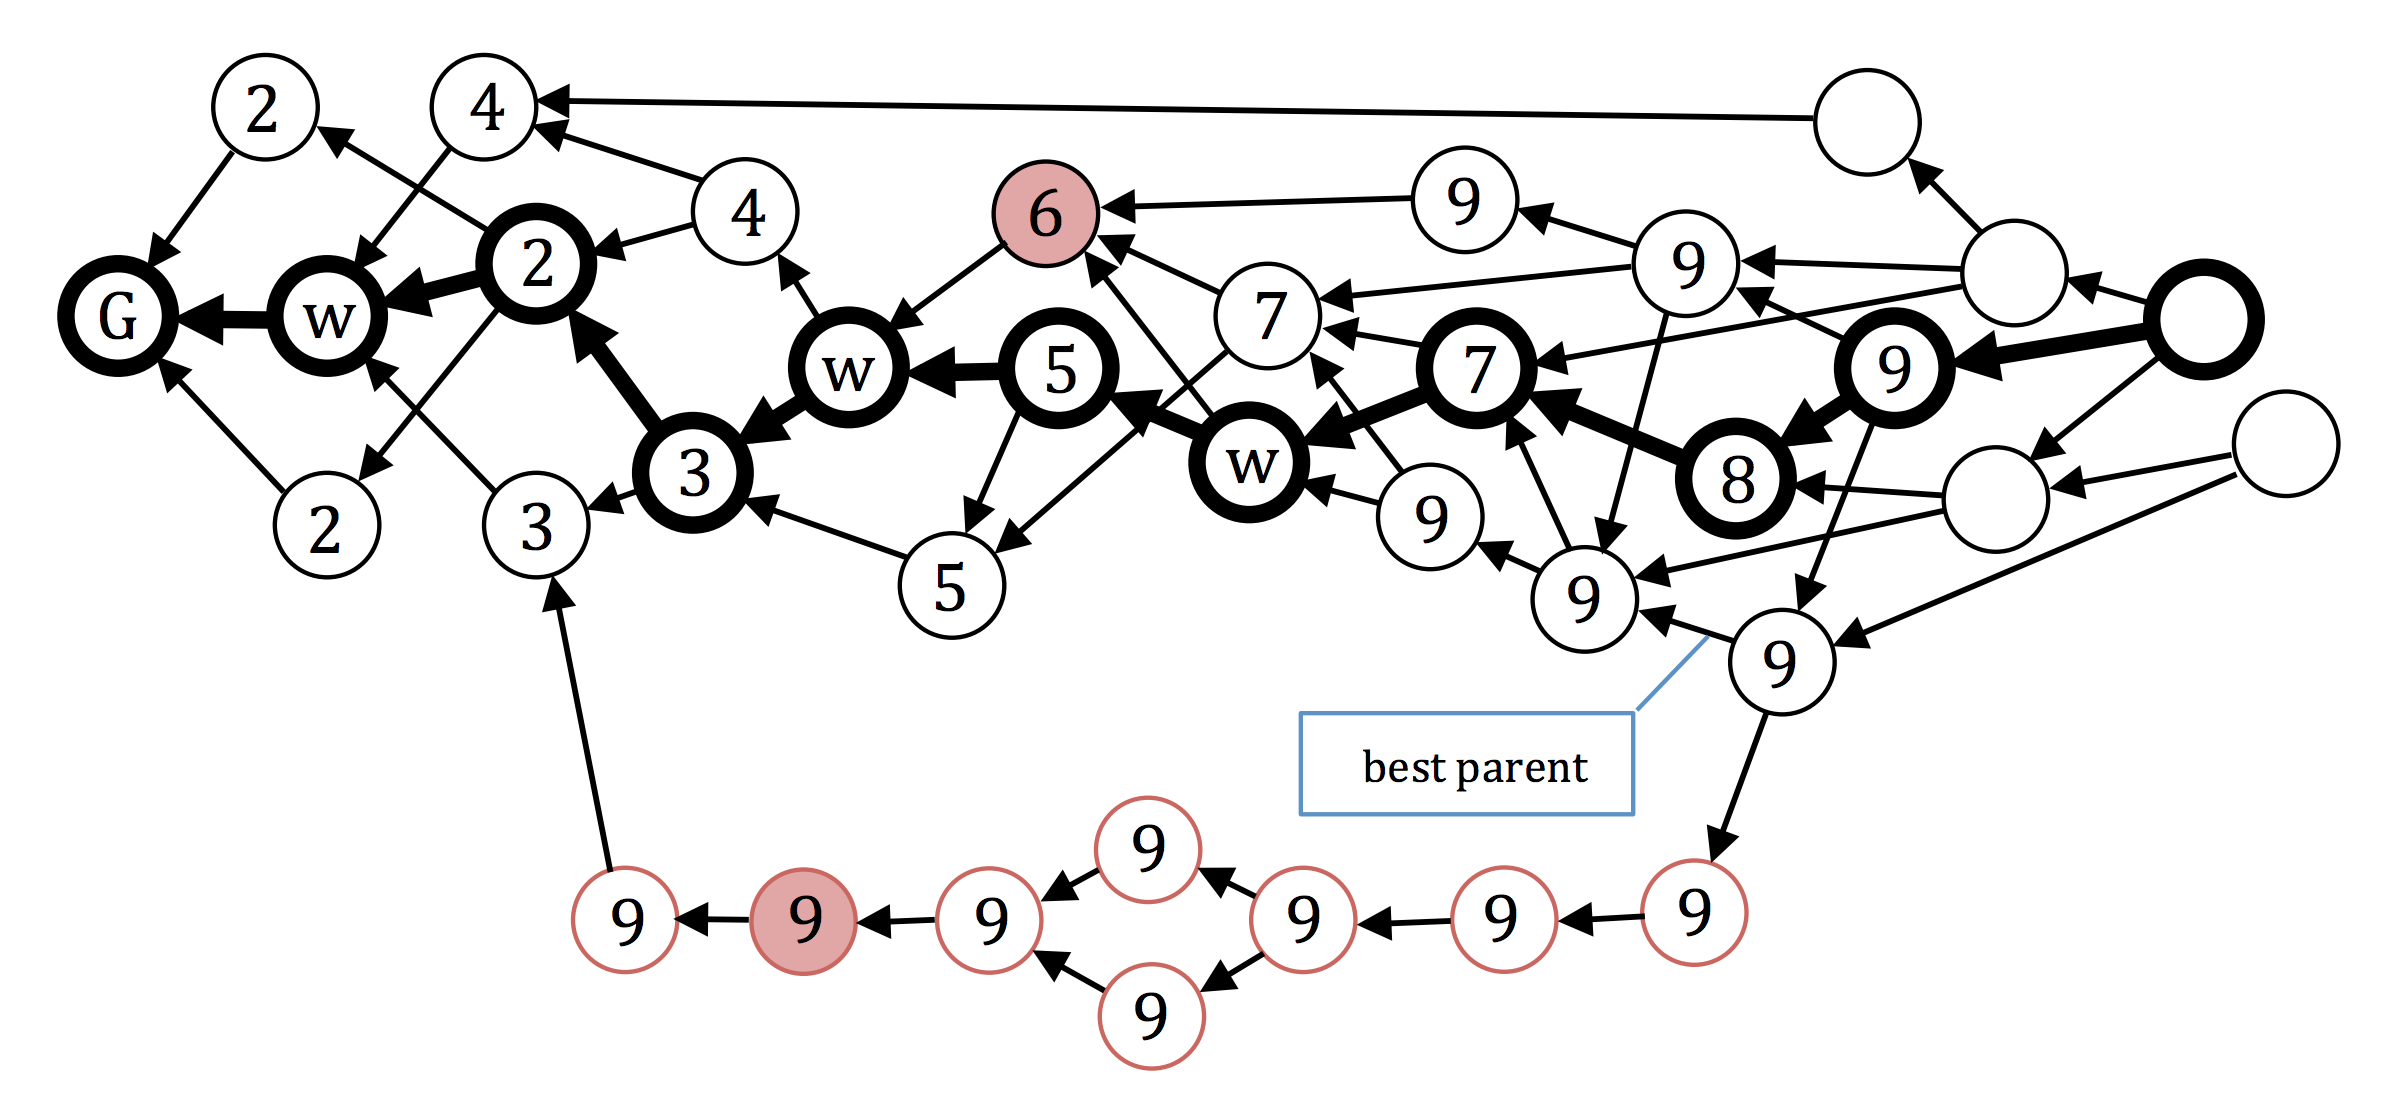
\includegraphics[width=\linewidth]{fig4.png}
  \caption{攻撃者がシャドウDAGを公開されているDAGに再統合する際、より多くのwitness(wで目印)がいる経路が優先されるため、最良の親の選択競争に敗れる。}
\end{figure}

この例は、witnessの過半数が順番決定済みのものだけを投稿すると信頼されていなければならない理由を示しています。過半数のwitnessは、攻撃者と共謀してシャドーチェーンに投稿してはいけません。私達がwitnessを信用すべきは、それが本物らしさのサインであり、いかなるシャドーチェーン上にも順番未決定ユニットを投稿しないという点のみであることに注意して下さい。私達は、彼らにネットワークやその一部でさえも支配権を与えることはありません。この小さな義務のためでさえも、witnessを指定するのはユーザーであり、ユーザーはいつでもその決定を変更することが出来ます。

本物らしさのサインとして、既知の実体を見るという考えは、新しいものではありません。特定の日付以前にデータが存在していたことを証明するために、データをハッシュ化して、印刷された新聞のような改変困難で広く目にされるメディアにそのハッシュを公開する方法は長い間知られており、一部の企業はそのような活動に従事しています[6]。Byteballのwitnessは新聞と同じ機能を果たします。新聞のように、彼らはよく知られており、信頼されるのです。新聞への信頼が与えられたデータを公開することに対する信頼のみに限定されるように、Byteballのwitnessは順番決定済みのものを投稿することに対してのみ信頼され、それ以上のものはありません。新聞のように、witnessは目撃しているハッシュの背後にあるものを知らず、気にする理由もほとんどありません。新聞は修正が難しい(ただし可能ではあり、『1984年』では実際に行われている)が、witnessによって作成された全てのものはデジタル署名で保護されているため、いかなる修正も不可能なのです。信頼性のために、私達にはたった一人ではなく複数のwitnessがおり、スピードと利便性のためにこれらはオンラインになっています。

witnessのリストを決めたら、「これらのwitnessが活動している場所」のような本物らしさの定義に最も適した親とそれに対応する履歴を選択することが出来ます。同時に、親自身が異なるwitnessのリストを持ち、結果として異なる本物らしさの定義を持つ可能性があります。私達は、本物らしさの定義、及びそれに紐づく履歴が何か共通のものに収斂することを望みます。これを達成するために、以下の追加のプロトコルルールを導入します。

「類似ルール」:最良の親は、子のwitnessリストと同じか1つのみ異なるwitnessリストを持つ親の中から選択されなければならない。このルールは、MC上の隣接ユニットのwitnessリストが十分に似ており、そのため、その履歴はお互いにほとんど一致することを保証します。witnessリストの違いが0または1の親は、(それらを直接含むユニットと)\emph{互換性がある}、他のものは互換性がないと呼ばれます。互換性のない親は依然許容されますが、最良の親になる機会はありません。もし、子が存在しないユニットの中に互換性のある親が存在しない場合(攻撃者は根本的に異なるwitnessリストを持つユニットでネットワークを溢れさせる可能性があります)、古いユニットから親を選択する必要があります。

上記は、各ユニットがそのwitnessを比較出来るようにリスト化しなければならないことを意味します。witnessの数は正確に12人でなければなりません。この12という数は以下の理由で選択されました:

\begin{itemize}
    \item 時折発生する数名のwitnessに対する障害から保護するのに十分な大きな数である(witnessが不正であったり、ハッキングされたり、または長い間オフラインになったり、秘密鍵を失って永久にオフラインになる可能性があります)。
    \item 人々が全てのwitnessを追跡して、誰が誰かを確認したり必要に応じてリストを変更することが出来るほどに十分に小さな数である。
    \item 許可された1人のwitnessの違いは、11人の変更されていないwitnessと比較して十分に小さな数である。
\end{itemize}

ユーザーがwitnessのいずれかが信頼性を失ったと考える場合や、単により良い候補者がいる場合は、witnessのリストを新しいリストと交換することが出来ます。ただし、witnessのリストが他のユニットと2つ以上異ならないように注意して下さい。これは、変化は徐々にしか起こらず、1つよりも大きな変化に対してはより一般的な合意が必要となることを意味しています。

\section{ファイナリティ}
新規ユニットが到着する度に、各ユーザーは自分にとっての\emph{現在のMC}を追跡します:これは、もし仮に現在の全ての子が存在しないユニットを基に新規ユニットを1つ発行した場合に形成されるであろうMCです。参照される子が存在しないユニットの集合はノード毎に異なる可能性があるため、現在のMCもノード間で異なる可能性があります。ここで現在のMCは、witnessリストに関わらず構築されるものとします。つまり、ユーザー自身のwitnessリストは問題にならず、例え互換性のない親でも最良の親に選択され得るとします。これは、例えば2人のユーザーが共通の子が存在しないユニットの集合を持ちながらも異なるwitnessリストを持つ場合、それでも彼らの現在のMCが同一となることを意味します。現在のMCは新規ユニットが到着する度に刻々と変化しますが、以下で論じるように、十分に古い部分に関しては不変となるのです。

私達はwitness(またはその過半数)が誠実に行動し、新規ユニットの投稿時には、1つ前に自身が署名したユニットを必ず含めることを期待しています。これは、witnessが新しいユニットを構成する時、直近のユニットのみが親として選ばれる候補であるということを意味します。従って、将来における全ての現在のMC群は、ある特定の安定点またはその手前(時間を遡って移動すると考えた場合の「手前」)で収束するはずなのです。つまり、ジェネシスユニットは初期の安定点ということになります。子が存在しないユニットの現状の集合に基づいて "現在のMC" を構築し、 そのMCには前々から安定的と思われる点、つまり将来の全ての現在のMCがそこかその手前 (再び強調するが時間を遡って移動すると考えた場合の 「手前」) で収束するであろう点が存在し、そして同じルートに沿って移動するものと仮定してみましょう。この時、もしこの点を前に進められる(ジェネシスユニットから遠ざかる)道を発見出来れば、帰納法によって安定点の存在を証明することが可能となります。

もし最良の親を除く全ての親を考慮外に置いた場合、DAGは最良の親へのリンクのみから成るツリーへと縮小される点に注意して下さい。当然のことながら、全てのMCはこのツリーの枝に沿います。安定点を次のMCIにまで進められるか否かを判断するためには、現在の安定点でツリーが分岐する場合としない場合の、2つのケースについて考える必要があります。

\begin{figure}[htbp]
  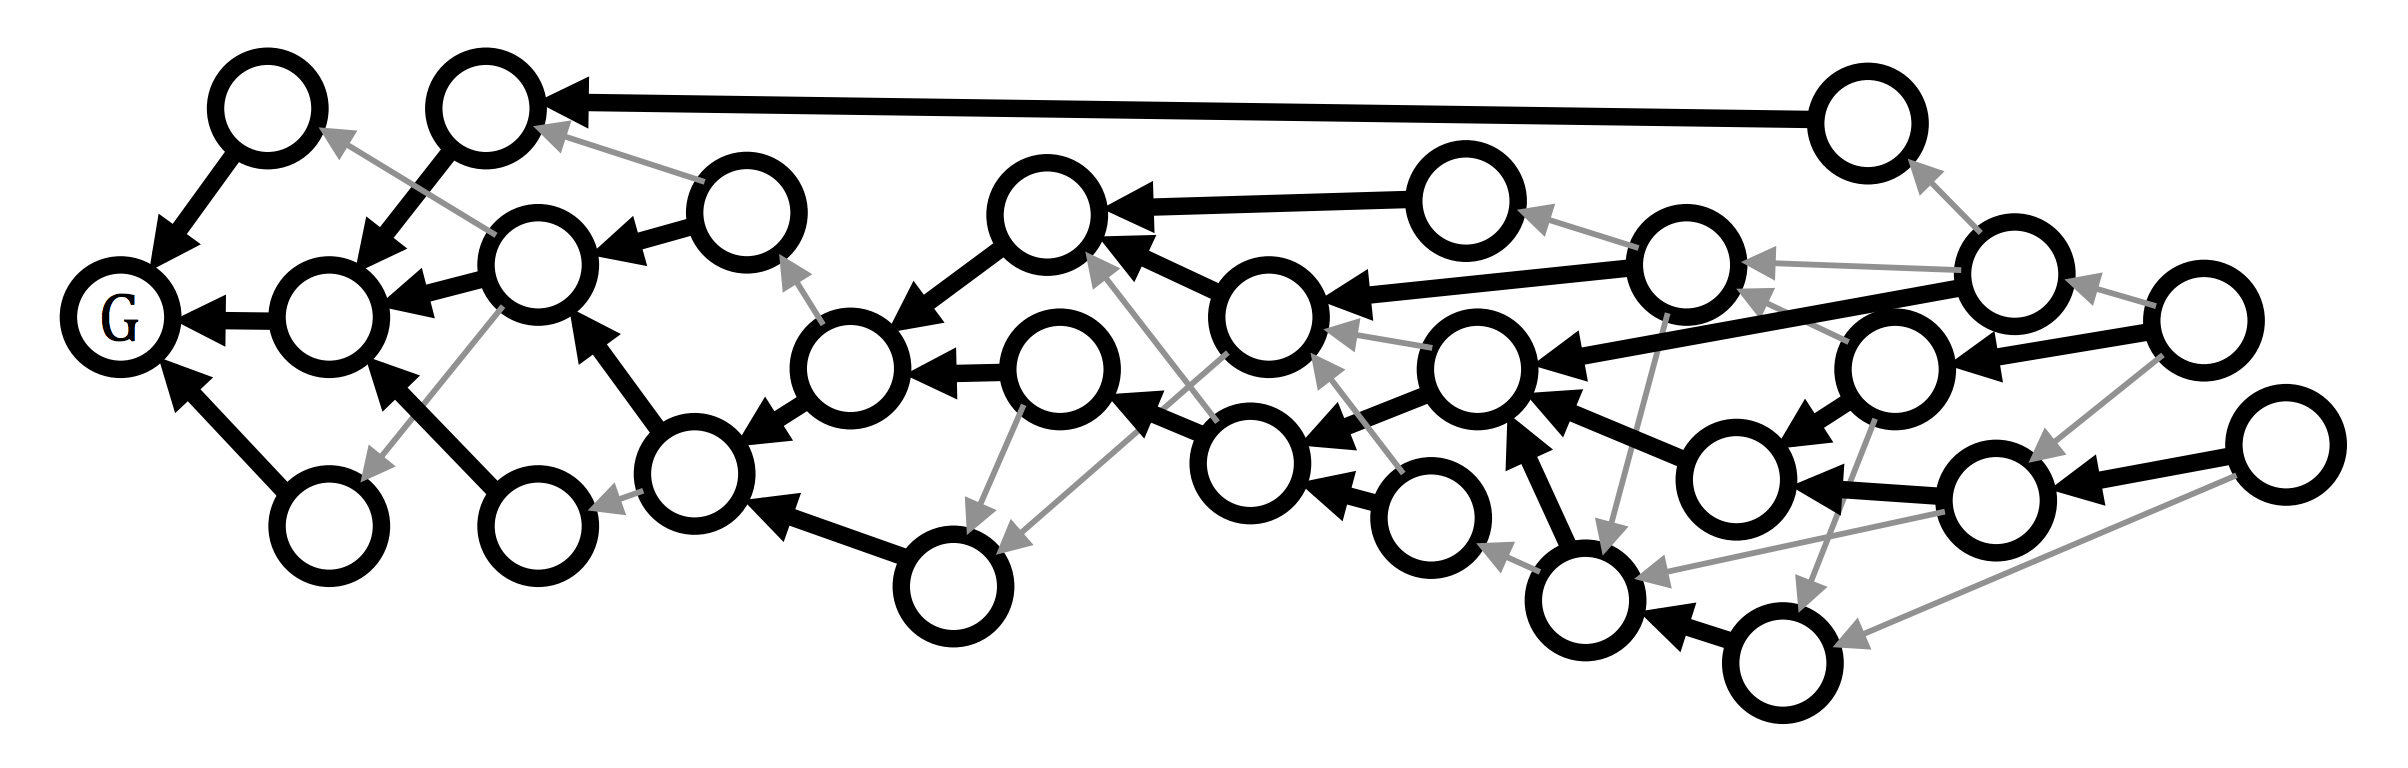
\includegraphics[width=\linewidth]{fig5.png}
  \caption{最良の親へのリンクから構成されるツリー。1つを除く全ての枝は、各々あるポイント以降で成長を止めている。}
\end{figure}

まずは、ツリーが分岐していないと仮定してみましょう。この場合、後に新たな分岐が発生し、その枝が何らかの理由によりwitness達に支持されることで既存の枝を超えて成長する可能性を考慮する必要があります。もう一方の可能性は、witness達が既存の枝を強く支持しており、以前のユニットを含めるという要件から今後も既存の枝を支持し続ける以外に選択肢が無いという状態です。後者の可能性を定量化してみましょう。親ノード群の中で最大のwitnessレベルを持つ物が最良の親に選ばれることを思い出して下さい。過半数のwitnessに出会うまで、現在のMCを先端部分から過去へと遡ってみましょう(witness達は、現在の安定点に存在するユニットによって定義されるものとします)。彼らのうちの少なくとも1つが現在の安定点より前に存在する場合、私達は安定点を前進させることはありません。存在しない場合には、前進させます。この場合、これらの全てのwitnessは、既に現在のMC中に「包含」されています。これらのwitness達の中で、最小のwitnessレベルであるmin\textunderscore wlを見つけます。これらのwitness達のいずれかが新しいユニットを投稿すると、このユニットは、そのMCが現在のMCにつながる親や、そのMCが競合する枝につながっている親を含む可能性があり、witnessレベルが最も高い親が最良の親として選択されて次の現行MCの方向を定義します。witnessは以前のユニットを含める必要があるため、現在のMCにつながる親のwitnessレベルは少なくともmin\textunderscore wlになるのです。たとえ全ての残った(少数の)witnessが別の枝に集まったとしても、別の枝につながるいかなる親のwitnessレベルも現在の安定点のレベルを超えることは決してありません。従って、もし現在のMCが十分に成長してmin\textunderscore wlが現在の安定点のレベルよりも大きくなると、witnessの過半数は既存の現行MCへの支持を増やさなければならなくなり、別の枝は全ての勝つチャンスを失い、安定点を次のMCIに移動することが出来るようになるのです。

次に、ツリーが分岐していると仮定します。私達は、別の枝が現在のMCを超えて成長する可能性が一切なくなるための条件を見つける必要があります。前の例のようにmin\textunderscore wlを定義することから始めましょう。別の枝の全てのユニットの中で、私達はwitnessレベルが上昇するもの、すなわち自身のwitnessレベルが全ての親のレベルよりも大きいもの、を選択します。これらの中で、私達は最大のwitnessレベルを見つけます。そして、たとえ全ての残った(少数の)witnessが別の枝に集まっても、その枝のwitnessレベルは決してこの最大レベルを超えることはありません。従って、この最大レベルがmin\textunderscore wlより小さい場合、別の枝はゲームオーバーとなり、私達は現在のMCに沿って安定点を進めることが出来るのです。

このように、(witnessの過半数が順番未決定ユニットを投稿しないとすると)現在のMC上にはそこより前のMCが決して変更されない安定点が存在します。従って、このMCに関連して定義される全順序もまた最終的なものなのです。もし順番未決定ユニットがあった場合、どちらが有効であるかの決定も同様に最終的なものとなります。もし安定したMC上のユニットと衝突する新しい順番未決定ユニットが出現した場合、その新しい順番未決定ユニットはすでに存在するもう一方の後となるように明確に順序付けされ、その新たなユニットは無効とみなされるでしょう。このように、安定したMC上に含まれるユニットによって作られる全ての支払いは、既に不可逆的です。トランザクションのファイナリティが確率論的でしかないBitcoinとは異なり、決定論的なのです。

全てのユーザーは、自身が見ているユニットに基づいて、自身の(主観的な)現在のMCを構築します。新しいユニットの伝播は即時的ではなく、異なるユーザに異なる順序で到着しうるため、ユーザーはいつでも異なるMCを持ち、MC上の最新の安定点について異なる見解を有します。しかし、現在のMCはユーザーに知られている一連のユニットによってのみ定義されるので、ユーザーBがユーザーAと同じMCIに安定点をまだ進めていない場合でも、後に必ず同じMCIに安定点を進めます - ユーザーAと同じかより多くのユニットを受け取るとすぐに。このように、任意のユニットの状態に関する異なるユーザの見解は、最終的に一致することになるのです。

\section{順番未決定ユニットの保存}
あるユニットが順番未決定となった場合でも保存は行われますが、その場合データの一部はハッシュへと置き換えられます。このルールには2つの目的があります。 1つは、支払い処理の無いユニットが消費するストレージ量を削減すること(順番未決定ユニットの中身は、手数料支払いを含む全体が無効とみなされます)、そしてもう1つは、ユーザーがこのようなユニットを送信しようとする効用を無くすことです(署名者がただ乗りで保存を試みた有用なデータは全てハッシュに置き換わってしまいます)。これにより、攻撃者が大量のデータを無料で保存する手法として順番未決定ユニットを悪用することを防ぎます。

ユニットの中身全体の保存にハッシュを代用した場合でも、オリジナルデータを手元に保管しておけばその存在証明としてハッシュは活用可能なので、その点において未だ効用は存在します。ただし:
\begin{enumerate}
        \item どのみちユニットが有効とみなされるためには(順番未決定とならないために)支払いが必要である。
        \item もし攻撃者が既にByteballデータの読み取りに必要なメタデータを内部に保存しているならば、所持している全データをマークルツリーに結合し、そのマークルルートのみをByteballへ保存しておけば、1つの小さなユニットにかかるコストのみで同様の目的が達成可能である。
\end{enumerate}

ため、この設計の下ではわざわざ順番未決定ユニットの送信を試みることに利益はありません。また、順番未決定ユニットは発見された段階で拒否出来る類の物では無いということにも言及しておかねばならないでしょう。もし拒否する場合、自作の順番未決定ユニットを異なるユーザー達へ異なる順序で送りつけるという攻撃手法が可能となります。

この場合ユーザー達は最初に受け取った方のバージョンに固執してもう一方のバージョンに基づく全てを拒否するようになるため、攻撃によってネットワークが分断されてしまいます。これが、まずは両バージョンを共に保存してその後に順序を決める理由です。さらにこの場合、その存在を他へと速やか知らせたほうが良いため、ユーザーは順番未決定ユニットに対しても通常ユニットと同様にピア達へ転送を行います。

それでも可能であるならば、順番未決定ユニットがネットワークへ含まれる事態は回避すべきでしょう。よって親選択のアルゴリズムは、順番未決定ユニットを子ユニットを持たない限り候補から除外するように設計されています。この点からも、出来る限り速くピア達に順番未決定ユニットの存在を知らせることが望ましいのです。

\section{Balls}
ユニットが安定した(すなわち、MCの安定的な部分に含まれた)後は、このユニットに基づいた\textit{ボール}と呼ばれる新しい構造体が作成されます:

\begin{lstlisting}[basicstyle=\ttfamily\footnotesize, frame=none]
ball: {
    unit: "hash of unit",
    parent_balls: [array of hashes of balls based on parent units],
    is_nonserial: true, // this field included only if the unit is nonserial
    skiplist_balls: [array of earlier balls used to build skiplist]
}
\end{lstlisting}

\noindent 各ボールは自身にとっての祖先である全てのボールに関する情報を(親を介して)含むため、それが依存する情報量は雪だるま式に増加していきます。またボールには、それが無効(順番未決定)であるかどうかを知らせるためのフラグ、そしてライトクライアントにも参照関係を示すために将来用いられる過去のボールへのレファレンスも含まれています。

ボールは、対応するユニットが安定し、かつ順番決定済であることに確証が得られた場合にのみ作成されます。異なるユーザー視点での現在のMCも最終的には一致するようになるので、各MCは全員同じユニットに基づき全く同じボールを作るはずです。

\section{最終ボール}
ボールの改ざんを防ぐ(特に is\textunderscore nonserial フラグの改ざん防止は最重要)ために、各新規ユニットは署名者が把握している最終ボールのハッシュを含まねばなりません (最終ボールとは、最新の安定したユニットから生成され、かつMC上にあるボールを表します)。この方法により、最終ボールは新規ユニット作成者の署名によって保護されるのです。そしてその後、新規ユニット自身もwitnessによって(直接的または間接的に)ハッシュへ含まれることになります。

もしByteball全体のデータベースを持っていない誰かがある特定のユニットについて順番決定済かどうかを知りたい場合、まずは自身が正直に行動していると信頼するwitnessリストの提示を行います。システムはこれを受け、提示されたwitness達の過半数を含む直近のユニットに関するチェーンを作成し、そのチェーンにおける最も古いユニットが含んでいる最終ボールを読み込みます。そして読み込んだボール群を用いて、最終ボールを頂点にリクエストされたユニットが下部のどこかに含まれるであろうハッシュツリーを作成します。このハッシュツリーは、各ノードに追加データが入力された非常に高いマークルツリーと類似した構造で、ツリーはスキップリストを使用して最適化することが可能です。

最終ボールを参照することで、ユーザーはMCの安定点についてピア達がどのように考えているかを確認し、自身のビジョンと比較することも出来ます。

また、自身の最終ボールは親にとっての最終ボール以後に存在せねばなりません。これは、最終ボールはMCに沿って前進するか同じ位置に留まるかのどちらかで、決して後退しないということを保証します。

攻撃相手の自由度をさらに減らすために、ここでもう1つ要件を追加します:あるユニットのwitnessリストは、そのユニットにとってのMCの後半部分(自分と最終ボールのユニットとの間)に存在する各ユニットのwitnessリストと互換性がなければなりません。この要件は、witnessリストに対する全ての変更を、別の変更が試みられる前にまず安定点へ到達させることを保証します。さもなくば、攻撃者が大幅に変更されたwitnessリストをMCへ紛れ込ませ、新しいwitnessアドレスからの投稿を止めてしまうことが起こり得ます。こうなると安定点は攻撃者の用意したwitnessが占有してしまった区間を超えて前進することが出来ません。

同時期に存在するユニットのwitnessリストがほぼ同じでなければならないという要件は、現時点においてコミュニティの灯台として誰が信頼出来るかについて、全てのユーザーがほぼ同じ意見を持っていることを意味します。これは同じ種の生物がほとんど同じ遺伝子を持たなければならない生物学と似ています。witnessリストの小さな変異は、システムの誠実さを保つ進化的変化を可能にするのです。

\section{witnessリストユニット}
以上の条件下では、多くのユーザーが全く同じwitnessリストを使用したがることが期待されます。この場合、スペース節約のために12人全員分のwitnessアドレスは記載せず、代わりにユーザーはwitness達が明示された先行する別ユニットへの参照を用います。
この対象となるwitnessリストユニットは、参照する側のユニット視点で安定的、すなわち、最終ボールのユニットに含まれていなければなりません。

\section{ユニット構造}
以下がユニットの一例です:
\begin{lstlisting}[basicstyle=\ttfamily\footnotesize, frame=none]
{
    version: `1.0',
    alt: `1',
    messages: [ {
        app: `payment',
        payload_location: `inline',
        payload_hash:
        `AegecfpDzh8xvdyIABdynrcP6CTd4Pt42gvRiv0Ftjg=',
        payload: {
            inputs: [{
                unit:
                `7yctnKyuAk5P+mFgFQDdDLza88nkceXYjsTs4e3doQA=',
                message_index: 0,
                output_index: 1
            } ],
            outputs: [
                { address: `DJ6LV5GPCLMGRW7ZB55IVGJRPDJPOQU6', amount: 208 },
                { address: `Z36JFFX2AH7X5JQ2V2C6AQUUOWFESKZ2', amount: 3505 }
            ]
        }
    } ],
    authors: [ {
        address: `DJ6LV5GPCLMGRW7ZB55IVGJRPDJPOQU6',
        authentifiers: {
            r:
            `3eQPIFiPVLRwBwEzxUR5thqn+zlFfLXUrzAmgemAqOk35UvDpa4h
            79Fd6TbPbGfb8VMiJzqdNGHCKyAjl786mw=='
        }
    } ],
    parent_units: [
        `B63mnJ4yNNAE+6J+L6AhQ3EY7EO1Lj7QmAM9PS8X0pg=',
        `D6O1/D9L8vCMhv+8f70JecF93UoLKDp3e2+b92Yh2mI=',
        `ZxqzWP6q6hDNF50Wax8HUK212lH/KSIRdW5a6T9h3DM='
    ],
    last_ball: `8S2ya9lULt5abF1Z4lIJ4x5zYY9MtEALCl+jPDLsnsw=',
    last_ball_unit: `bhdxFqVUut6V3N2D6Tyt+/YD6X0W+QnC95dMcJJWdtw=',
    witness_list_unit:
    `f252ZI2MN3xu8wFJ+LktVDGsay2Udzi/AUauE9ZaifY='
}
\end{lstlisting}

\noindent ここで:
\begin{itemize}
    \item versionはプロトコルのバーション番号です。ユニットはこのプロトコルのバージョンに従って読み取られます。
    \item altは代替通貨の識別子です。これについては後に説明します。
    \item messagesは実データを含む1つ以上のメッセージの配列です。
    \begin{itemize}
        \item appはメッセージの種類です。例えば支払いの場合は`payment'、任意のテキストメッセージの場合は`text'などが存在します。
        \item  payload\textunderscore locationはメッセージのペイロードがどこにあるのかを示します。ペイロードがメッセージに含まれている場合は`inline'、インターネットアドレスで利用可能な場合は`url'、全く公開されていない場合は`none'が存在し、非公開で記録及び/または共有されます。また、payload\textunderscore hashがペイロードが特定の時間に存在したことを証明する役割を果たします。
        \item payload\textunderscore hashはbase64エンコーディングでのペイロードのハッシュです。
        \item payloadは実際のペイロードです(例では`inline'の場合を示しています)。 ペイロードの構造はapp毎に異なり、支払いの場合には以下のように記述されます:
        \begin{itemize}
            \item  inputsは支払時に入力として消費されるコインに関する配列です。入力コインの全ての所有者は、ユニットの署名者達の中にいなければなりません。
            \begin{itemize}
                \item unitは入力コインの出所となったユニットのハッシュです。支払い可能となるためには、このユニットがlast\textunderscore ball\textunderscore unitに含まれていなければなりません。
                \item message\textunderscore indexは出所となった入力ユニットのメッセージ配列に関するインデックスで、入力ユニットに含まれるどのメッセージが出所になったかを示します。
                \item output\textunderscore indexは入力ユニットにおけるmessage\textunderscore index番目のメッセージのoutputs配列に関するインデックスで、コインの出力先を示します。
            \end{itemize}
            \item outputsは誰がお金を受け取るかを示す出力先に関する配列です。
            \begin{itemize}
                \item addressは受取人のByteballアドレスです。
                \item amountは受取金額です。
            \end{itemize}
        \end{itemize}
    \end{itemize}
    \item authorsはこのユニットを作成し署名を行った署名者の配列です。全ての入力コインは、この作者達に属していなければなりません。
    \begin{itemize}
        \item addressは署名者のByteballアドレスです。
        \item authentifiersは署名者の真正性を示すためのデータ構造です。ほとんどの場合、ECDSA署名が用いられます。
    \end{itemize}
    \item parent\textunderscore unitsは親ユニットのハッシュからなる配列です。この配列はアルファベット順にソートされていなければなりません。
    \item last\textunderscore ballとlast\textunderscore ball\textunderscore unitはそれぞれ、最終ボールとそのユニットのハッシュです。
    \item witness\textunderscore list\textunderscore unitはwitnessリストを参照したユニットのハッシュです。
\end{itemize}

\noindent 全てのハッシュは、base64エンコーディングです。

ここで、ユニット構造にタイムスタンプフィールドが無い点に注意して下さい。Byteballには、時刻に依存するプロトコルが存在しません。イベントの順序だけに頼れば十分であるため、単純に不必要なのです。

それでもタイムスタンプは、ノードからノードへ転送される時にユニットへ追加されます。しかしこれはあくまで補助的なもので、長時間のオフラインによりユニットの受取時間が大きく異なってしまう可能性があるライトクライアント用に、ユニットが作成されたおおよその時間をウォレットに表示するため使用されます。


\section{手数料}
前述の通り、ユニットを保存する際のコストはbytes換算での容量です。手数料は、ヘッダー手数料とペイロード手数料という2つの部分に分割されます。ペイロード手数料はメッセージ部分の容量と等しく、ヘッダー手数料は他全ての容量です。この2種類の手数料は、異なる方法で分配されます。

ヘッダー手数料は、それを支払ったユニットを親にした将来のユニットの1つへ充てられます。この時、受取人は手数料を支払ったユニットのMCIとその次のMCIの両方が安定的になった後に初めて選択されます。受取人を決定するために、まずは手数料を支払ったユニットとMCIが同じまたは1つ大きな子ユニット達を選定します。これら子ユニット達のハッシュはそれぞれ個別に(手数料を支払ったユニットから見て)次のMCI上にあるユニットのハッシュと連結され、その返り値の中で最小のハッシュ値(16進数)を持つ子ユニットがヘッダー手数料を獲得するのです。 次のMCユニットと合体させるハッシュ化は(次のMCユニットを事前に知り得ないため)その値が予想出来ず、よって自身のユニットハッシュをいじくり回しても手数料獲得の可能性を高めることが出来ないように設計されています。同時に、候補者をMCIが同じまたは1つだけ大きなユニットに制限することは、直近のユニットを親として選択することへのインセンティブにもなります。これは、DAGの幅を出来るだけ狭く保つのに効果的です。

すぐに親に選んでくれた子ユニットに対しては、以下の理由により、手数料全体では無くヘッダー手数料のみが支払われます。もし手数料全体を支払う場合、データを複数のチャンクに分割しそれらを1つずつユニットへ格納することによって自身のユニットのみで長いチェーンを作成すると言った、制度の乱用を誘発するでしょう。この時、前のユニットで支払われた手数料全体は、次のユニットも作っている同じユーザーがすぐに回収してしまいます。ヘッダー手数料のみの支払いにすることで、チェーンに新しい要素を追加するためには獲得出来る金額とほぼ同額のヘッダー手数料を支払わなければならなくなるので、このような行動は割に合わなくなります。残りの(ペイロード)手数料は、ネットワーク全体を健全に保つために重要な活動を行う他のユーザー達へのインセンティブとして使用されます。

ペイロード手数料は、witness達に充てられます。witness達が十分頻繁に投稿するインセンティブを与えるために、ペイロード手数料は、手数料を負担したユニットの後100MCI以内に投稿を行った全てのwitnessに対し平等に分割されます(witnessが速く投稿する程、ユニットが安定化するのも速くなります)。つまりもし12人のwitness全員がこの期間内に投稿した場合、各witnessはペイロード手数料の1/12を受け取り、反対にもし1人のwitnessしか投稿しなければ、そのwitnessがペイロード手数料を総取りするのです。 また、期間内にどのwitnessも投稿しなかったという特殊なケースでは、witness達全員でペイロード手数料を1/12ずつ受け取ります。加えて、もし分割時に端数が出た場合には数学的ルールに従って四捨五入されます。この調整のためにwitnessへ支払われるペイロード手数料の合計とユニット署名者が負担するペイロード手数料の合計は必ずしも一致せず、総供給量も僅かに変化します。そして当然のことながら、手数料の分配は 手数料負担ユニットのMCI+100 が安定した後に限り行われます。

獲得したヘッダー手数料や witnessing(ペイロード)手数料を支払いに用いる際には、以下のinputsが使用されます:

\begin{lstlisting}[basicstyle=\ttfamily\footnotesize, frame=none]
inputs: [
    {
        type: "headers_commission",
        from_main_chain_index: 123,
        to_main_chain_index: 196
    },
    {
        type: "witnessing",
        from_main_chain_index: 60,
        to_main_chain_index: 142
    },
    ...
]
\end{lstlisting}

このinputsは、from\textunderscore main\textunderscore chain\textunderscore indexとto\textunderscore main\textunderscore chain\textunderscore index間のMCIで発行され手数料を支払ったユニット群から、署名者が獲得した全てのヘッダー及びwitnessing(ペイロード)手数料分を収集します。当然のことながら、to\textunderscore main\textunderscore chain\textunderscore indexは安定的でなければなりません。

複数人によって署名されたユニットがヘッダー手数料を得た場合、署名者間で手数料をどのように分割するかはこれまで曖昧にしていました。この曖昧さを取り除くためには、複数人によって署名された各ユニットは収入の分配比率が記述されたデータ構造を含まなければなりません:

\begin{lstlisting}[basicstyle=\ttfamily\footnotesize, frame=none]
unit: {
    ...
    earned_headers_commission_recipients: [
    {address: "ADDRESS1", earned_headers_commission_share: 30},
    {address: "ADDRESS2", earned_headers_commission_share: 70}
    ],
    ...
}
\end{lstlisting}

手数料を受け取るアドレスはユニット署名者のアドレスと同じである必要は無く、よって手数料はどのアドレスにも送ることが可能です。また、例えユニットの署名者が1人の場合でも、この入力フィールドを含むことでヘッダー手数料を他の宛先へとリダイレクトすることが出来ます。


\section{承認時間}
承認時間とは、あるユニットがデータベースへ格納されてから安定性を確保するまでの時間です。 安定的となるには、新しく追加されたユニットの後にMCに沿ってwitness署名ユニットが十分に蓄積される必要があるため、承認時間はwitnessが投稿を行う頻度に依存します。この時間を最小限に抑えるために、witnessにはやり過ぎない程度に頻繁な投稿が求められます(そのために手数料の分配ルールを通じたインセンティブが与えられています)。もし2人以上のwitnessがユニットをほぼ同時(そのユニットが他のwitnessに伝播する時間よりも速く)に発行した場合、最良の親のリンクからなるツリーに不必要な分岐が発生し、安定的になるまでの時間が遅くなってしまいます。このような理由から、witness達が十分に連携しかつ高速なマシンで運営され、新たなユニットの妥当性をすぐに検証出来る場合に、最短の承認時間が達成されます。私達は、この最短の承認時間を30秒前後と見積もっています。これは、新規ユニットの流入が十分に多く、ゆえにwitness達がユニットの投稿にかかる費用以上の手数料収入を得られる場合にのみ達成可能な水準です。

完全な承認までの時間は長いものの、ピア達が全ての新規ユニットをフィルタリングせずに配信してくれると信頼するノードにとっては、一旦ユニットが1人のwitnessに含まれ、さらに典型的な待ち時間(ある新規ユニットがピアからピアへ移動するのにかかる時間)が経過すれば、そのユニットはほとんどの場合ファイナリティが得られ有効とみなされるはずです。たとえ後に二重支払いが発生したとしても、そのユニットの順序はこのユニットよりも後に置かれる可能性が高いでしょう。

\section{分割リスク}
Byteballノードのネットワークでは、2つの部分に分割されたことに気付かず双方が運用され続けることは決してありません。例えヨーロッパとアメリカを結ぶ大西洋ケーブルが切断されたと言った世界的なネットワーク混乱の事態でも、少なくとも分割された一方の側はwitnessの過半数を失ったことに気付くことでしょう。つまりそちらの側では安定点は前に進まず、誰もMCの不安定な部分に詰まったoutputを送金することが出来なくなるのです。もし誰かが二重支払いを試みても、接続が回復するまでは不安定な状態(従って認識されない状態)のままです。witnessの大部分が残っているもう一方の側においては、通常通りの運用が続きます。

\section{検閲}
設計上、Byteballでは過去の記録を変更または消去することは既に不可能です。また、特定のタイプのデータがデータベースに入ることを止めるのも非常に困難です。

まず、データ自体は秘匿しそのハッシュのみを実際にデータベースへ投稿する場合でも、データが存在していたことは証明出来ます。元データは、ハッシュが格納されたユニットが他のユニットに含まれて改訂不可能となった後にようやく公開されることでしょう。

さらに、例えデータが公開されていても、それをデータベースに含めるか否かの決定は対応する新規ユニットを親として扱うであろう(実際そうなるようなインセンティブが与えられています)無数の匿名ユーザ達に委任されています。望ましくないユニットに対して検閲を試みる人は、それらを直接(親として)含むことのみならず、他のユニットを通じて間接的に含むことも回避せねばなりません。(これはマイナーやマイニングプールが個人のトランザクションを直接フィルタリング出来、現にそれが行われているBitcoinとは異なります。 さらに、Bitcoinユーザーには誰がマイナーになるべきかに関する発言権がありません) 「不都合な」ユニットを含んでいるユニットの数が雪だるま式に増えるにつれて、それを回避する試みそのものに検閲が必要となるでしょう。コンテンツに対して実効性のある禁止ルールを課すことが出来るのは、witnessの多数派のみなのです – もしユーザーがそのようなwitness達を選ぶならば。

\section{witnessの選択}
witness達への信頼はByteballを現実の世界に根ざしたものにしています。同時に、人間の意思決定に大きく依存するようにもしています。システムの健全性は信頼に足るwitnessのリストを責任持って設定するユーザー達に依存するのです。このプロセスは、安全に自動化することが出来ません。例えばもしほとんどのユーザーが互換性を保つべく直近確認したユニットのリストと一致するように自らのwitnessリストを自動更新する場合、攻撃者はユニットを氾濫させることでネットワーク上で支配的なwitnessリストを自分が望むものへと徐々に変更出来てしまうため、システムは簡単に攻略されてしまいます。

最も推奨するのは「手動でwitnessリストを編集する」ことなのですが、これは多くのユーザーにとって非常に負担になるでしょう。witnessリストの管理に対するより現実的なアプローチとは、ネットワークの健全性を大切に思っていたり、あるいはByteballとは必ずしも関係しない活動でも良い評判を得ている "captains of industry" 数名のwitnessリストを追い、何らかの方法で平均化することです。 彼らの中にはwitnessとして活動する者もいるかもしれません。witnessリストとは異なり、captains of industryのリストは互換性を必要とせず、このリストを十分頻繁に更新しなかったからといって、互換性のある親を見つけられずに新規ユニットが投稿出来ないなどの悪影響がすぐに引き起こされる訳ではありません。ほとんどのユーザーがいくつかの人気のあるウォレットの中から1つを使用し、それらのウォレットではベンダーのwitnessリストが既定値となっており、そしておそらくベンダーは他の著名なプレイヤーのリストを見ている、というのが好ましい状態です。

witness達も自分のwitnessリストを持っており、ユーザーが選出するwitness達は、このリストを一般ユーザーの信条を代弁する状態で維持してくれるであろう人物が相応しいでしょう。現在のwitness達の過半数が承認しなければネットワーク上で支配的なwitnessリストを変更することは出来ないため、これは非常に重要です。witness及びその候補者達が自身のwitnessリストに関するポリシー(他の評判の高いユーザーのリストに従う、あるいは平均化するなど)を公に宣言し、ユーザー達は彼らの適正をこのポリシーやその他の要素に基づいて評価する、という状態が推奨されます。宣言されたポリシーに対するいかなる違反もすぐ目に見えるようになるので、それがwitness交代キャンペーンを引き起こすこともあり得るでしょう。ポリシーの不当な改正についても同様です。このポリシーは、例え世論がwitnessやwitness支持者達に反対するようになった場合でも、witnessが世論に従うよう制約するのです。

既に述べたように、プロトコルルールは以下を必要とします:
\begin{enumerate}
    \item 最良の親は、witnessリストの差異が1以下の親達からのみ選択される。
    \item 最終ボールユニットのwitnessリストとの間の差異は、1以下でなければならない。
    \item 最終ボールユニットに至るまでの不安定なMCユニット全てのwitnessリストとの間の差異は、1以下でなければならない。
    \item 安定点は、(現在の安定点によって定義された)witness達がその安定点の後に十分な数のユニットを投稿した場合にのみ前進する。
\end{enumerate}

\noindent これらのルールは、悪意のある分岐や偶発的な分岐からの保護を目的としています。同時に、支配的なwitnessリストの変更は段階的に成されねばならず、各ステップには現在のwitness達の過半数の承認が必要であることも示唆しています。リスト内のある1箇所を変更した場合、それが安定点に到達し以前のwitness達の過半数に認識されない限り、別の変更に着手することは出来ません。もし2名のwitnessを直ちに交代する必要があるとコミュニティが突如判断した場合、MC上への変更が1回行われた後、最初の変更が安定するまで、上記のルール3により2回目の変更がブロックされます。

以上全ての推奨事項にもかかわらず、industry leadersの過失により、選ばれたwitness達が後にカルテルを形成し、witness手数料から得られる利益を維持するために、その中の誰か一人を交代するような試みを協力して全てブロックするということも依然として起こり得ます。witness達のこのような行動は、他のほとんどのindustry leadersのwitnessリストが(互換性を保つ最大許容量である)差異1で異なる一方で、彼らのリストは変更されないままなので、誰の目にも明らかとなります。このような明白な圧力にもかかわらず古いwitness達が役を譲らない場合、変化を望むユーザー達の唯一の頼りとは「革命」です。すなわち、古いコインのある時点からの全ての残高やユーザーアドレスなどを継承しつつも、新たなwitnessリストから開始され、かつ分裂の瞬間にこの互換性の無い変化を処理するための特別なプロトコルルールが加えられた新規コインを始めるのです。古いコインと区別するためには、`alt'フィールドに新しい値を割り当て(これこそが`alt'の役割です)新規コインの下で発行された全てのユニットにそれを使用します。この結果、ユーザーは2種類のコイン(古いコインは alt= "1", 新しいコインは例えば alt= "2" など)を持ち、双方独立した支払いを行えるようになるでしょう。もし分割した側が正当となった場合、古いコインは放棄される可能性がありますが、分裂前に蓄積された全てのデータは新規コインで通常通り利用可能となります。また(分裂とaltの変更を処理するためのルールを除く)プロトコルはほぼ同一であるため、全てのユーザー及び業者の端末にインストールされているソフトウェアは簡単に更新出来るでしょう。

単に別のプロトコルルールの実験として新規コインを始めたい場合も、実験者は`alt'フィールドを用いることによって、古いコインの全てを継承し、ユーザーのコイン間のスイッチを快適にし、かつ残高を持つ大量のユーザー達をその日の内に獲得することが可能です。

\section{スキップリスト}
いくつかのボールには、ライトクライアント用に証明を素早く行うためのスキップリスト配列が含まれています(下記参照)。これを保持しているのは、MC上に直接あり、かつMCIが10で割り切れるボールのみです。スキップリストには、MCI末尾に自分と同じあるいは少ない数のゼロを持ち、かつ最も近くにある以前のMCボール群が各々掲載されています。例えば MCI 190 のボールには、MCI 180 のボールを参照するスキップリストが存在します。そして MCI 3000 のボールは、MCI 2990, 2900, 2000のボールを参照するスキップリストを持ちます。

\section{ライトクライアント}
ライトクライアントは、Byteballのデータベース全体を格納しません。代わりに、いずれかのユーザーアドレスが入出金を行っているトランザクションといった、関心あるデータの部分集合のみをダウンロードします。

ライトクライアントは、関心のあるユニットをダウンロードするためにフルノードへ接続し、信頼するwitness達のリスト(新規ユニットを作成する際に用いるwitnessと必ずしも同じである必要はありません)と自分のアドレス群のリストをフルノードに伝えます。そしてフルノードは、ライトクライアントが興味を持っているユニット群を検索し、以下の方法で各ユニットのプルーフチェーンを構築します:
\begin{enumerate}
    \item 提示されたwitness達の過半数が現れるまでMCの時系列を遡り、そこに至るまでの全てのMCユニットを集める。
    \item この集合における最後のユニット(時間的に言えば最も早いユニット)から、最終ボールを読み込む。
    \item この最終ボールから、スキップリストを持つボールに出会うまでMCの時系列を遡り、そこに至るまでの全てのボールを集める。
    \item スキップリストを利用して、それが参照する以前のボールの1つへとジャンプする。このボールもスキップリストを持っているため、再びジャンプする。スキップリスト配列に複数のボールがある場合には、常に最大限可能な距離だけジャンプする。つまり最初に10個、次に100個、次に1000個ずつとジャンプは加速して行く。
    \item もし次のスキップリストによるジャンプで目的のボールを飛び越える場合、ジャンプの距離を小さくすることによって減速する。最終的にはスキップリストから離れ、親リンクのみを辿ってMCIを1つずつ遡る。
\end{enumerate}

\noindent このチェーンはまず初めにwitnessが署名したユニット群を持つことによってライトクライアントの観点から信頼出来るものとなり、またチェーンの全要素は(witnessを蓄積する間に通った)親ユニットのリンク、最終ボールの参照、親ボールのリンク、スキップリストのリンクのいずれかによってリンクされています。そしてチェーンの最後に、その存在を証明すべきであった目的のユニットが置かれています。

\section{マルチシグ}
ユニットは複数の関係者によって署名することが出来ます。その場合、ユニット内のauthors配列は2つ以上の要素を持つことになります。

これは、2人以上の関係者がコントラクト(スマートなものではなく、単純な従来のコントラクト)に署名したい場合などで役に立つでしょう。両者ともテキストメッセージ(app=`text')を含む同一のユニットに署名します。この時、コントラクトの全テキストを料金を払って公開データベースに保存する必要はありません - ハッシュで十分であり(payload\textunderscore location=`none')、関係者達はテキストを非公開の状態で保管することが出来ます。

マルチシグの別の応用はアセットの交換です。ユーザーAがアセットXをアセットYとの交換でユーザーBに送ろうとしていると仮定しましょう(ネイティブ通貨 `bytes' もアセットの1つであり、システムにおける基本アセットです)。この場合、彼らは2つのpaymentメッセージを含むユニットを構成します:一方はアセットXをAからBへ送るため、もう一方はアセットYをBからAに送るためのものです。この2名によって作成されたユニットは、両者が共に署名することで公開されます。交換はアトミック、つまり両方の支払いが同時に実行されるか同時に失敗するかのどちらか、となります。一方の支払いが二重支払いと思われる場合、ユニット全体が無効となり、もう一方の支払いも無効とみなされます。

このシンプルな構造により、ユーザーは集中型取引所にお金を信託することなくアセットを直接交換することが出来ます。

\section{アドレス}

ユーザーはアドレスによって識別され、トランザクションoutputはアドレスに送られます。そして、Bitcoinのように、ユーザーは複数のアドレスを持ち、再利用を避けることが推奨されます。しかし場合によっては、再利用することが普通です。例えば、witnessは同じアドレスから繰り返し投稿するのが望ましいでしょう。

アドレスはブール式で示される定義を表します(Bitcoinスクリプトに若干似ています)。ユーザーはユニットに署名する際に、認証データの一式(authentifiers、通常ECDSA署名)も提供します。その認証データは、定義に適応される際に、このユーザーが署名する権利があることを証明するために、真と評価されなければならないものです。定義はJSONに記述します。例えば、これは1つのECDSA署名を必要とするアドレスの定義です:

\begin{lstlisting}[basicstyle=\ttfamily\footnotesize, frame=none]
["sig",{"pubkey":"Ald9tkgiUZQQ1djpZgv2ez7xf1ZvYAsTLhudhvn0931w"}]
\end{lstlisting}

\noindent 定義は、アドレスの所有者が(base64エンコードされた)定義内で与えられた公開鍵に対応する秘密鍵を持つことを示し、所有者はこの秘密鍵で全てのユニットに署名します。上記の定義は、対応するauthentifierで与えられた署名が有効である場合は真と評価され、そうでない場合は偽となります。署名はauthentifiersを除く全てのユニットのデータに対して計算されます。

所与の定義オブジェクトに対応するアドレスは、初期定義オブジェクトにチェックサムを加えたもののハッシュに過ぎません。チェックサムは入力エラーを回避するために追加されます。しかし、一般的な設計とは異なり、チェックサム用のビットはデータの末尾のみならず、内部の複数箇所に挿入されます。この設計により、アドレスを入力すべき箇所に不正なデータの長い文字列を挿入することが困難になります。また、アドレスはbase32エンコーディングで記述されます。以上の定義は次のようなアドレスに対応します:A2WWHN7755YZVMXCBLMFWRSLKSZJN3FU

アドレスに資金を入れる時、支払いの送付者は支払いoutputにアドレス(定義のチェックサム付きハッシュ)のみを認識し指定します。outputが使用されるまで定義は公開されず、所有者以外の誰からも不明なままです。

ユーザーがアドレスから最初のユニットを送信する時、署名の検証を可能にするためにauthors配列内で定義を公開しなければなりません:

\begin{lstlisting}[basicstyle=\ttfamily\footnotesize, frame=none]
unit: {
    ...
    authors: [ {
        address: `DJ6LV5GPCLMGRW7ZB55IVGJRPDJPOQU6',
        definition: [
            "sig",
            {"pubkey":"AsnvZ3w7N1lZGJ+P+bDZU0DgOwJcGJ51bjsWpEqfqBg6"}
        ],
        authentifiers: {
            r:
            `3eQPIFiPVLRwBwEzxUR5thqn+zlFfLXUrzAmgemAqOk35UvDpa4h
            79Fd6TbPbGfb8VMiJzqdNGHCKyAjl786mw=='
        }
    } ],
    ...
}
\end{lstlisting}

ユーザーが同じアドレスから2番目のユニットを送信する場合は、定義(Byteball上で既知)を省略する必要があります。ユーザーは定義が安定しなければ2番目のユニットを送信することが出来ません。すなわち、2番目のユニットの最後のボールユニットは定義が公開されたユニットを含まなければなりません。

ユーザーは古いアドレスを保持しつつアドレスの定義を更新することが出来ます。例えば、アドレスにリンクされた秘密鍵を入れ替えるには、ユーザーは次のようなメッセージを含むユニットを投稿する必要があります:

\begin{lstlisting}[basicstyle=\ttfamily\footnotesize, frame=none]
unit: {
    ...
    messages: [
        ...
        {
            app: "address_definition_change",
            definition_chash: "I4Z7KFNIYTPHPJ5CA5OFC273JQFSZPOX"
        },
        ...
    ],
    ...
}
\end{lstlisting}

\noindent ここで、definition\textunderscore chashは新しいアドレス定義(まだ公開されていないもの)のチェックサム付きハッシュを示し、ユニット自体は古い秘密鍵によって署名されなければなりません。このアドレスの次のユニットは以下を満たす必要があります:

\begin{itemize}
    \item その最後のボールユニットにaddress\textunderscore definition\textunderscore changeを含みます。すなわち、既に安定したものでなければなりません。
    \item アドレスからの最初のメッセージと同様にしてauthors配列の新しい定義を公開します。
\end{itemize}

変更後は、アドレスは現在の定義のチェックサム付きハッシュとは異なります。一方、最初の定義のチェックサム付きハッシュとは等しいままです。

定義の変更は、ユーザーが古いアドレスを保持したまま鍵を変更したい時(例えば、新しいデバイスに移行する時)に便利です。例えばこのアドレスが既に長く使われている定義に関係している場合です(下記参照)。

\subsection{定義構文}

\subsubsection{論理演算子}
定義には“and”条件を含めることが出来ます。例:

\begin{lstlisting}[basicstyle=\ttfamily\footnotesize, frame=none]
["and", [
    ["sig", {pubkey: "one pubkey in base64"}],
    ["sig", {pubkey: "another pubkey in base64"}]
]]
\end{lstlisting}

\noindent これはトランザクションに署名するために、ノートPCとスマートフォンのような2つの独立したデバイスからの署名が必要な場合に便利です。

“or”条件は次のようになります:

\begin{lstlisting}[basicstyle=\ttfamily\footnotesize, frame=none]
["or", [
    ["sig", {pubkey: "laptop pubkey"}],
    ["sig", {pubkey: "smartphone pubkey"}],
    ["sig", {pubkey: "tablet pubkey"}]
]]
\end{lstlisting}

これはユーザーがデバイスのいずれかから同じアドレスを使用したい場合に便利です。条件は入れ子にすることが出来ます:

\begin{lstlisting}[basicstyle=\ttfamily\footnotesize, frame=none]
["and", [
    ["or", [
        ["sig", {pubkey: "laptop pubkey"}],
        ["sig", {pubkey: "tablet pubkey"}]
    ]],
    ["sig", {pubkey: "smartphone pubkey"}]
]]
\end{lstlisting}

定義にはある集合の中で満たさなければならない最小の条件数を要求することも出来ます。例、2-of-3署名:

\begin{lstlisting}[basicstyle=\ttfamily\footnotesize, frame=none]
["r of set", {
    required: 2,
    set: [
        ["sig", {pubkey: "laptop pubkey"}],
        ["sig", {pubkey: "smartphone pubkey"}],
        ["sig", {pubkey: "tablet pubkey"}]
    ]
}]
\end{lstlisting}

\noindent (“r”は“required”を表す)2つの署名を必須とするセキュリティと信頼性の両方の特性を持つため、1つの鍵を紛失した場合でもアドレスは使用可能であり、定義を変更して紛失した3つ目の鍵を新しいものに入れ替えることが出来ます。

また、それぞれの条件に異なる重みを与えて、必要とする最小値を設定することが出来ます:

\begin{lstlisting}[basicstyle=\ttfamily\footnotesize, frame=none]
["weighted and", {
    required: 50,
    set: [
        {weight: 40, value: ["sig", {pubkey: "CEO pubkey"}] },
        {weight: 20, value: ["sig", {pubkey: "COO pubkey"}] },
        {weight: 20, value: ["sig", {pubkey: "CFO pubkey"}] },
        {weight: 20, value: ["sig", {pubkey: "CTO pubkey"}] }
    ]
}]
\end{lstlisting}

\subsubsection{他のアドレスへの委任}
アドレスは他のアドレスへの参照を含むことが出来ます:

\begin{lstlisting}[basicstyle=\ttfamily\footnotesize, frame=none]
["and", [
    ["address", "ADDRESS 1 IN BASE32"],
    ["address", "ADDRESS 2 IN BASE32"]
]]
\end{lstlisting}

\noindent これは、他のアドレスに署名を委任し、共同で管理されるアドレス(複数のユーザーによって制御される)を構築する場合に便利です。この構文のおかげで、ユーザーは他のユーザーに迷惑をかけることなく、自身の構成アドレスの定義をいつでも柔軟に変更することが出来ます。


\subsubsection{署名とauthentifiers}
ほとんどの場合、定義には少なくとも1つの署名が(直接的または間接的に)含まれます:

\begin{lstlisting}[basicstyle=\ttfamily\footnotesize, frame=none]
["sig", {pubkey: "pubkey in base64"}]
\end{lstlisting}

署名の代わりに、定義にはハッシュを与えるための原像が必要な場合もあります:

\begin{lstlisting}[basicstyle=\ttfamily\footnotesize, frame=none]
["hash",{"hash":"value of sha256 hash in base64"}]
\end{lstlisting}

\noindent これはクロスチェーン取引アルゴリズム [7] に使用出来ます。この場合、ハッシュの原像はauthentifiersの1つとして入力されます。

既定の署名アルゴリズムはsecp256k1曲線のECDSAです(Bitcoinと同じ)。最初からサポートされている唯一のアルゴリズムです。将来的に量子セキュアNTRUアルゴリズムなどの他のアルゴリズムが追加されると、定義の該当部分でアルゴリズム識別子が使用されます:
\begin{lstlisting}[basicstyle=\ttfamily\footnotesize, frame=none]
["sig", {algo: "ntru", pubkey: "NTRU public key in base64"}]
\end{lstlisting}

マルチシグネチャ定義により、実証されていない署名スキームを、従来の署名と組み合わせて安全に試すことが出来ます。

ユニットヘッダーのauthentifiersオブジェクトは署名や、アドレス定義内の認証要求サブ定義のパスに合わせた他のデータ(ハッシュ原像など)を含みます。シングルシグアドレス

\begin{lstlisting}[basicstyle=\ttfamily\footnotesize, frame=none]
["sig", {pubkey: "pubkey in base64"}]
\end{lstlisting}

\noindent の場合、パスは単に“r”です(rはrootを表す)。認証要求サブ定義が他の定義(and/orなど)に含まれる場合、パスはインデックスによってこのサブ定義が含まれる配列の中に拡張され、パス構成はドットで区切られます。例えば、アドレスの定義は次のようになります:

\begin{lstlisting}[basicstyle=\ttfamily\footnotesize, frame=none]
["and", [
    ["sig", {pubkey: "one pubkey in base64"}],
    ["sig", {pubkey: "another pubkey in base64"}]
]]
\end{lstlisting}

\noindent パスは“r.0”と“r.1”です。深く入れ子にされた定義の場合:

\begin{lstlisting}[basicstyle=\ttfamily\footnotesize, frame=none]
["and", [
    ["or", [
        ["sig", {pubkey: "laptop pubkey"}],
        ["sig", {pubkey: "tablet pubkey"}]
    ]],
    ["sig", {pubkey: "smartphone pubkey"}]
]]
\end{lstlisting}

\noindent パスは“r.0.0”と“r.0.1”と“r.1”です。2-of-3のような選択可能な署名がある場合、パスはどの鍵が実際に使われたのかを示します。

\subsubsection{定義テンプレート}
定義は定義テンプレートを参照することも出来ます:

\begin{lstlisting}[basicstyle=\ttfamily\footnotesize, frame=none]
["definition template", [
    "hash of unit where the template was defined",
    {param1: "value1", param2: "value2"}
]]
\end{lstlisting}

\noindent パラメータはテンプレート内で置換する変数の値を指定します。テンプレートは、特別なメッセージタイプapp=’definition\textunderscore template’で事前に保存しておく必要があります(また通常は、使用前に安定している必要があります)。テンプレート自体はメッセージペイロードにあり、テンプレートは通常の定義のように見えますが、構文に変数@param1、@param2への参照を含む場合があります。定義テンプレートはコードの再利用を可能にします。それらは他のテンプレートを参照することもあります。

\subsubsection{連署}
サブ定義はユニットを他のアドレスによる連署を要するようにすることも出来ます:

\begin{lstlisting}[basicstyle=\ttfamily\footnotesize, frame=none]
["cosigned by", "ANOTHER ADDRESS IN BASE32"]
\end{lstlisting}

\subsubsection{アドレスが使用されているかどうかのクエリ}
サブ定義のもう1つの可能な要件:最新のボールユニットに含まれるユニットのうち少なくとも1つのユニットにおいて、アドレスが署名者としてみなされること:

\begin{lstlisting}[basicstyle=\ttfamily\footnotesize, frame=none]
["seen address", "ANOTHER ADDRESS IN BASE32"]
\end{lstlisting}

\subsubsection{データフィード}
過去にByteballに格納されたデータのクエリを作成するために非常に便利な条件があります:
\begin{lstlisting}[basicstyle=\ttfamily\footnotesize, frame=none]
["in data feed", [
    ["ADDRESS1", "ADDRESS2", ...],
    "data feed name",
    "=",
    "expected value"
]]
\end{lstlisting}

\noindent この条件は、リストされたアドレス"ADDRESS1", "ADDRESS2", ..(オラクル)によって署名されたデータフィードメッセージの中で、"data feed name"と"expected value"が等しいメッセージが少なくとも1つある場合に真と評価されます。データフィードは次のようなメッセージタイプです:

\begin{lstlisting}[basicstyle=\ttfamily\footnotesize, frame=none]
unit: {
    ...
    messages: [
        ...
        {
            app: "data_feed",
            payload_location: "inline",
            payload_hash: "hash of payload",
            payload: {
                "data feed name": "value",
                "another data feed name": "value2",
                ...
            }
        },
        ...
    ],
    ...
}
\end{lstlisting}

データフィールドはオラクルに関する定義の設計に使用出来ます。2人以上の当事者が特定のエンティティ(オラクル)が正しいデータを提供すると信用している場合、共同で管理するアドレスを設定し、オラクルによって投稿されたデータに応じて当事者達に異なる権利を与えることが出来ます。例えば、このアドレス定義はバイナリオプションを表します:

\begin{lstlisting}[basicstyle=\ttfamily\footnotesize, frame=none]
["or", [
    ["and", [
        ["address", "ADDRESS 1"],
        ["in data feed", [["EXCHANGE ADDRESS"], "EURUSD", ">",
        "1.1500"]]
    ]],
    ["and", [
        ["address", "ADDRESS 2"],
        ["in data feed", [["TIMESTAMPER ADDRESS"], "datetime", ">",
        "2016-10-01 00:00:00"]]
    ]]
]]
\end{lstlisting}

\noindent 初めに、二人の当事者がこの定義のアドレスに資金を提供します(信用要件を排除するためにマルチシグを使用し、両方の当事者によって署名されるシングルユニットで賭け金を送ります)。EXCHANGE ADDRESSで発行されたEUR/USDの為替レートが1.1500を超えると、1人目の当事者が資金を独占出来ます。2016年10月1日までにそれが起こらず、タイムスタンプオラクルがそれ以降の日付を投稿した場合、2番目の当事者がこのアドレスに格納されている全ての資金を独占出来ます。両方の条件が真でありアドレス残高が空でない場合、両方の当事者が同時にその資金を取り出そうとする場合があります。その場合の二重支払いは通常通り解決されます。

比較演算子は "=", "!=", ">", ">=", "<", "<=" が使用出来ます。データフィードメッセージは通常のように最後のボールユニットの前に来る必要があります。唯一のオラクルが前触れなくオフラインになるリスクを軽減するために、複数のフィード提供者アドレスをリストすることが出来ます。

別の例として、客が業者から商品を購入しようとしているが、その業者をあまり信用しておらず、商品が配達されない場合は返金してもらいたいという場合があります。客は次のように定義された共有アドレスに支払います:

\begin{lstlisting}[basicstyle=\ttfamily\footnotesize, frame=none]
["or", [
    ["and", [
        ["address", "MERCHANT ADDRESS"],
        ["in data feed", [["FEDEX ADDRESS"], "tracking", "=",
        "123456"]]
    ]],
    ["and", [
        ["address", "BUYER ADDRESS"],
        ["in data feed", [["TIMESTAMPER ADDRESS"], "datetime", ">",
        "2016-10-01 00:00:00"]]
    ]]
]]
\end{lstlisting}

\noindent 定義は、配達が完了した全ての荷物のトラッキングナンバーを投稿するFedExオラクルに依存します。荷物が配達されると、業者は1つ目の条件を用いてお金をアンロックすることが出来ます。指定された日付までに配達されない場合、客はお金を取り戻します。

この例は、FedExが全ての個別の荷物について投稿しなければならないためやや普通ではありません。

\subsubsection{マークル・データ・フィード}
同じ結果を得るためのより現実的な方法として、別の構文があります:

\begin{lstlisting}[basicstyle=\ttfamily\footnotesize, frame=none]
["in merkle", [
    ["ADDRESS1", "ADDRESS2", ...],
    "data feed name",
    "hash of expected value"
]]
\end{lstlisting}

これは、期待値の指定ハッシュが、"ADDRESS1", "ADDRESS2",... からデータフィードに投稿されたマークル根に含まれている場合、真と評価されます。この構文を用いると、FedExは前回の投稿以降に完了した全ての荷物のマークル根を定期的に投稿するだけです。このアドレスから支払うために、業者は指定された値が対応するマークル木に確かに含まれていることを証明するマークルパスを提供する必要があります。マークルパスはauthentifiersの1つとして提供されます。


\subsubsection{自己点検}
定義はユニット自身へのクエリを含むことが出来ます。

\begin{lstlisting}[basicstyle=\ttfamily\footnotesize, frame=none]
[`has', {
    what: `input'|`output',
    asset: `assetID in base64 or "base" for bytes',
    type: `transfer'|`issue',
    own_funds: true,
    amount_at_least: 123,
    amount_at_most: 123,
    amount: 123,
    address: `INPUT OR OUTPUT ADDRESS IN BASE32'
}]
\end{lstlisting}

\noindent このサブ定義ではユニットが、全ての指定されたフィルターを通過するような少なくとも1つの(`what' フィールドに応じて)inputまたはoutputを持つ場合に真と評価されます。全てのフィルターはオプションです。

類似の条件 `has one' はフィルターを通過するinputまたはoutputがちょうど1つあることを要件とします。

条件 `has' は分散型取引所を構築するために使用することが出来ます。これまでに、マルチシグのアセット交換への使用について議論してきました。

しかし、マルチシグだけでは価格交渉の仕組みがありません。1,000 bytes以下で1,200単位の別のアセットを買いたいというユーザーを仮定しましょう。また、彼は売り手を待つ間、常にオンラインであるわけではありません。むしろ彼は取引所に注文を出すだけで、合致する売り手が現れた時に注文を実行させたいと考えています。ここで定義されたアドレスに1,000 bytesを送ることで指値注文を作成することが出来ます:

\begin{lstlisting}[basicstyle=\ttfamily\footnotesize, frame=none]
["or", [
    ["address", "USER ADDRESS"],
    ["and", [
        ["address", "EXCHANGE ADDRESS"],
        ["has", {
            what: "output",
            asset: "ID of alternative asset",
            amount_at_least: 1200,
            address: "USER ADDRESS"
        }]
    ]]
]]
\end{lstlisting}

\noindent 1つ目のor条件分岐は、ユーザーが好きな時にbytesを取り戻して注文をキャンセル出来るようにします。2つ目の条件分岐は、資金を使用する権利を取引所に委任し、同じユニットにおいて少なくとも1,200単位の別のアセットをユーザーのアドレスに支払うという別のoutputを提供します。取引所はオーダーのリストを公開し、それを見た売り手はアセットを交換するユニットを構成し、取引所とマルチ署名を行います。

‘has’ 条件を使用することで担保付きのレンディングも可能です。非流動的なアセットを保有している借り手がbytes(またはその他の流動的なアセット)を必要としているとしましょう。この時借り手と貸し手は1つのユニットにマルチ署名することが出来ます。ユニットの一部は必要とするbytesを貸し手に送信し、ユニットの他の部分は非流動的なアセットを次のように定義されるアドレスにロックします:

\begin{lstlisting}[basicstyle=\ttfamily\footnotesize, frame=none]
["or", [
    ["and", [
        ["address", "LENDER ADDRESS"],
        ["in data feed", [["TIMESTAMPER ADDRESS"], "datetime", ">",
        "2017-06-01 00:00:00"]]
    ]],
    ["and", [
        ["address", "BORROWER ADDRESS"],
        ["has", {
            what: "output",
            asset: "base",
            amount: 10000,
            address: "LENDER ADDRESS"
        }]
    ]],
    ["and", [
        ["address", "LENDER ADDRESS"],
        ["address", "BORROWER ADDRESS"]
    ]]
]]
\end{lstlisting}

\noindent 1つ目のor条件分岐により、期間内にローンが返済されなかった場合に貸し手は担保を差し押さえることが出来ます。2つ目の条件分岐により、借り手は貸し手に10,000 bytes(利子を含む合意済みのローンサイズ)の支払いを行うことで担保を取り戻すことが出来ます。3つ目の条件分岐により、両者が合意した場合に条件を改定することが出来ます。

また、以下の条件をサブ定義に含めることが出来ます:

\begin{lstlisting}[basicstyle=\ttfamily\footnotesize, frame=none]
[`has equal', {
    equal_fields: [`address', `amount'],
    search_criteria: [
        {what: `output', asset: `asset1', address: `BASE32'},
        {what: `input', asset: `asset2', type: `issue', own_funds:
        true, address: `ANOTHERBASE32'}
    ]
}]
\end{lstlisting}

\noindent これは、検索条件を満たすinputまたoutputのペア(ペアの1つ目の要素は1番目のフィルタセットによって検索され、2つ目は2番目によって検索されます)が少なくとも1つあり、そのフィールドの一部が等しい時に真と評価されます。

類似条件の ‘has one equal’ はそのようなペアがちょうど1つだけあることを要件とします。

もう1つのサブ定義は一定の条件でフィルタリングされたinputまたはoutputの合計をターゲット値と比較することが出来ます:

\begin{lstlisting}[basicstyle=\ttfamily\footnotesize, frame=none]
[`sum', {
    filter: {
        what: `input'|`output',
        asset: `asset or base',
        type: `transfer'|`issue',
        own_funds: true,
        address: `ADDRESS IN BASE32'
    },
    at_least: 120,
    at_most: 130,
    equals: 123
}]
\end{lstlisting}

\subsubsection{否定}
“sig”、“hash”、“address”、“cosigned by”、“in merkle” を含まない任意の条件は否定することが出来ます:

\begin{lstlisting}[basicstyle=\ttfamily\footnotesize, frame=none]
["not", ["in data feed", [["NOAA ADDRESS"], "wind_speed", ">",
"200"]]]
\end{lstlisting}

\noindent 新しいデータフィード投稿が表示されないような非常に古い親を選ぶことも正当であるため、通常、上記のような否定条件とタイムスタンプが一定の日付以降であるような要件を組み合わせます。


\subsection{一般的な要件}
アドレス定義には少なくとも1つの “sig” が明示的または黙示的(例えば “address” など)に含まれている必要があります。

検証に使うリソースが大きくなりすぎないようにするために、操作の総数は “address” や “definition template” などの参照した定義の操作を含め、1定義あたり100までに制限されています。

この数字はByteball上の9個しかない任意定数の1つです。他の8個は:witnessの総数:12、witnessリストの最大許容差異:1、witness報酬用MCインデックスの最大数:100、ヘッダサイズのためにカウントされる親の数:2、ユニットあたりの最大メッセージ数:128、メッセージあたりの最大input/output数:128、ユニットあたりの最大署名者数:16、最大通貨供給量:$10^{15}$。比較のために、Bitcoinは少なくとも17の定数を持ち [8]、Ethereumは手数料表のためだけに30の定数を定義しています [9]。

上記の定義言語は宣言型であり、全体がブール式で構成されているため、従来の法的契約の言葉に近いものになっていることに注意して下さい。ただし、表現力においては、まだEthereumのスマートコントラクト言語に近い言語とは言えません。実際、それは簡単な ‘Hello world’ プログラムを書くことすら出来ません。これは私達の目標ではありませんでした。Byteballの定義言語は包括的なものとして設計されていません。むしろ、可能な限り多くの人に、プログラマーでなくても理解出来るように設計されています。そのわかりやすい構文により、誰でも解釈可能で、開発者(スマートコントラクトの時代の“弁護士”)の手助けがなくても単純な定義を構成出来るようになり、間違いが起こる可能性を最小限にします。


\section{プロフィール}
ユーザーは必要に応じてByteballにプロフィールを保存することが出来ます。それにはこのようなメッセージを使用します:

\begin{lstlisting}[basicstyle=\ttfamily\footnotesize, frame=none]
unit: {
    ...
    messages: [
        ....
        {
            app: "profile",
            payload_location: "inline",
            payload_hash: "hash of payload",
            payload: {
                name: "Joe Average",
                emails: ["joe@example.com", "joe@domain.com"],
                twitter: "joe"
            }
        },
        ...
    ],
    ...
}
\end{lstlisting}

\noindent 自身に関する開示データ量や正確さについては、ユーザー自身に委ねられます。ユーザーに関する特定の情報が真実であると保証するためには、証明書を探す必要があります。


\section{認証}

認証は、発行したユーザー(アテスター)が認証済みのユーザー(対象)に関して何らかのデータを検証したことを裏付けます。認証はこのようにメッセージに格納されます:

\begin{lstlisting}[basicstyle=\ttfamily\footnotesize, frame=none]
unit: {
    ...
    messages: [
        ...
        {
            app: "attestation",
            payload_location: "inline",
            payload_hash: "hash of payload",
            payload: {
                address: "ADDRESS OF THE SUBJECT"
                profile: {
                    name: "Joe Average",
                    emails: ["joe@example.com"]
                }
            }
        },
        ...
    ],
    ...
}
\end{lstlisting}

認証に含まれる情報はユーザーが自身で公開したプロフィールと一致する必要はありません。事実、自身で公開したプロフィールが存在しない場合もあります。

アテスターの仕事は現代の認証局の仕事に似ており、対象の実社会のアイデンティティを検証し、特定の公開鍵(またはByteballアドレス)が個人または団体に帰属していることを証明します。彼らはByteballで同じ活動を継続し、実社会とByteballにおけるアイデンティティの間の関係を証明したい人から手数料を取るものと考えられます。witnessとwitnessになろうとする人は、信頼を高めるために認証を必要とするでしょう。特定のアセットタイプでは、アセットの取引を行うために認証を必要とするものがあります(下記参照)。

認証が必要であるが、対象の名前は重要でないアプリケーションの場合、認証済みプロフィールにおいて名前やその他の個人情報を省略することが出来ます。認証済みプロフィールは対象に関する重要な情報を全く含んでいなくてもよく、従ってアテスター以外の全ての人に対して匿名性を保つことが出来ます。アテスターは対象に関する情報を保持し続け、アテスターの規約で定められたことや法律による要求などの特定の状況のもとで開示することがあります。


\section{アセット}
データベースはあらゆるデータの不変なストレージとして設計されました。あらゆるデータのクラスの中で、共通データベースのストレージにおいて最も興味深いことは、それが社会的価値を持つことです。即ち、データに1人や2人よりも多くの人にとって価値があるということです。そのようなクラスの1つがアセットです。アセットは不特定多数の人が保有することが出来、Byteballにおける不変性とイベントの全順序付けは、所有権移転の長いチェーンの妥当性を確立する上で非常に重要です。Byteball上のアセットは発行、移転、交換が可能であり、そしてネイティブ通貨"bytes"と同様に振る舞います。それらは、債権、株式、ロイヤルティポイント、放映枠、商品、他の法定通貨や暗号通貨など、あらゆる価値を表現することが出来ます。

新しいアセットを定義するには、定義するユーザーは以下のようなメッセージを送信します:

\begin{lstlisting}[basicstyle=\ttfamily\footnotesize, frame=none]
unit: {
    ...
    messages: [
        ...
        {
            app: "asset",
            payload_location: "inline",
            payload_hash: "hash of payload",
            payload: {
                cap: 1000000,
                is_private: false,
                is_transferrable: true,
                auto_destroy: false,
                fixed_denominations: false,
                issued_by_definer_only: true,
                cosigned_by_definer: false,
                spender_name_attested: true,
                attestors: [
                    "2QLYLKHMUG237QG36Z6AWLVH4KQ4MEY6",
                    "X5ZHWBYBF4TUYS35HU3ROVDQJC772ZMG"
                ]
            }
        },
        ...
    ],
    ...
}
\end{lstlisting}

\noindent ここで:
\begin{itemize}
    \item cap は発行可能な最大数量です。事前定義されたネイティブ通貨bytesの場合は、capは$10^{15}$です。
    \item is\textunderscore private はアセットの移転が匿名または公開で行われるかを指定します(以下参照)。bytesは公開です。
    \item is\textunderscore transferrable はアセットの定義者を経由せずに、第三者間で移転可能かどうかを指定します。移転可能でない場合、定義者は全ての移転において常に送信者であるか受信者である必要があります。bytesは移転可能です。
    \item auto\textunderscore destroy はアセットが定義者に送信された時に破棄されるかどうかを指定します。bytesは自動的には破棄されません。
    \item fixed\textunderscore denominations はアセットを任意の整数量(任意数量)で送信することが出来るか、紙幣や硬貨などのように決まった単位(例 1, 2, 5, 10, 20 など)でしか送信出来ないかを指定します。bytesは任意数量です。
    \item issued\textunderscore by\textunderscore definer\textunderscore only はアセットが定義者のみが発行出来るかどうかを指定します。bytesでは、全てのマネー供給がジェネシスユニットで発行されます。
    \item cosigned\textunderscore by\textunderscore definer は全ての移転がアセットの定義者によって連署される必要があるかどうかを指定します。これは規制アセットに便利です。bytesの移転には誰の連署も必要ありません。
    \item spender\textunderscore attested は使用者が使用に際して認証を必要とするかどうかを指定します。アセットを受け取ったがまだ認証受けていない人は、使用するためには定義に記載されたアテスターの一人の認証を受ける必要があります。この要件も規制アセットに便利です。bytesは認証を必要としません。
    \item attestors はアセット定義者によって認められたアテスターのアドレスのリストです(spender\textunderscore attested が有効の場合のみ)。定義者は ‘asset\textunderscore attestors’ メッセージを送信してアテスターのリストを置き換えることでリストを改訂することが出来ます。
    \item denominations(この例では表示されていません。fixed\textunderscore denominations アセットでのみ使用します)は、使用可能な全ての単位とそれぞれの単位で発行出来る総枚数のリストです。
    \item transfer\textunderscore condition はアセットの移転が許可される条件の定義です。定義は"sig"のようなauthentifierを必要とするものを参照出来ないという点を除けば、アドレス定義と同じ言語で書かれます。デフォルトでは、他のフィールドで定義済みのもの以外に制限はありません。
    \item issue\textunderscore condition は発行トランザクションに関する transfer\textunderscore condition と同様のものです。ユニットあたり、1「アセット」以下のメッセージでなければなりません。
\end{itemize}

定義後のアセットは、定義が行われたユニットのハッシュによって識別されます(そのため、1ユニットあたり1アセットである必要があります)。

アセットの移転はbytesの移転とほとんど同じですが、アセットIDの追加フィールドがあることだけ異なります:

\begin{lstlisting}[basicstyle=\ttfamily\footnotesize, frame=none]
unit: {
    ...
    messages: [
        ...
        {
            app: "payment",
            payload_location: "inline",
            payload_hash: "hash of payload",
            payload: {
                asset: "hash of unit where the asset was
                defined",
                inputs: [
                    {
                        unit: "hash of source unit",
                        message_index: 0,
                        output_index: 1
                    },
                    ...
                ],
                outputs: [
                    {
                        address: "BENEFICIARY ADDRESS",
                        amount: 12345
                    },
                ...
                ]
            }
        },
        ...
    ],
    ...
}
\end{lstlisting}

移転を可能にする前に、ユーザーは発行トランザクションを送信してアセットを作成します。発行トランザクションはinputのフォーマットが若干異なります:

\begin{lstlisting}[basicstyle=\ttfamily\footnotesize, frame=none]
unit: {
    ...
    messages: [
        ...
        {
            app: "payment",
            payload_location: "inline",
            payload_hash: "hash of payload",
            payload: {
                asset: "hash of unit where the asset was
                defined",
                inputs: [
                    {
                        type: "issue",
                        amount: 1000000,
                        serial_number: 1,
                        address: "ISSUER ADDRESS" // only
                        when multi-authored
                    },
                    ...
                ],
                outputs: [
                    {
                        address: "BENEFICIARY ADDRESS",
                        amount: 12345
                    },
                    ...
                ]
            }
        },
        ...
    ],
    ...
}
\end{lstlisting}

\noindent 上限付き任意数量アセットの総供給量は単一のトランザクションで発行される必要があります。特に、全てのbytesはジェネシスユニットで発行されます。アセットに上限が設定されている場合、発行のシリアルナンバーは必ず1です。上限が設定されていない場合、同一アドレスによる発行には、その都度固有のシリアルナンバーが付与されます。

アセットの定義は一度だけ作成することが出来、アテスターのリストを除いて後から修正する事が出来ません。

このアセットが何を表すものであるかは、定義者次第です。それが発行者の債権である場合、発行者は債権者の信頼を得るために、認証済みであるか匿名性を放棄するべきです。

エンドユーザーはアセットを使うことも使わないことも自由ですが、アセットの定義者はアセットに関係するトランザクションにあらゆる条件を課すことが出来ます。

様々なアセット特性を組み合わせることにより定義者は、規制金融機関が監視しなければならないものも含めた、幅広い要求を満たすアセットを考案することが出来ます。例えば、移転毎に定義者の連署を要件とする場合、金融機関は規制や契約条項に反する全ての支払いを効率的に拒否することが出来ます。それぞれの支払いへ連署する前に、金融機関(定義者かつ発行者)はユーザーが間違いなく顧客であること、資金の受取人もまた顧客であること、両顧客が本人確認(KYC)を済ませていること、資金が裁判所命令で差し押さえられていないことのチェック、及びアセットの定義後に導入されたものも含めた、絶えず変わり続ける法律、規制、社内規則によって要求されるその他のチェックを実施することが出来ます。

\subsection{銀行発行アセット}
銀行は法令に完全準拠したセキュリティをもつため(また、全ての資金移転が決定論的なファイナリティを保証されているため)、国の通貨にペッグされ、銀行の資産に裏付けされたアセットを発行することが出来ます(中央銀行によって適切に監査・監視されています)。そのようなアセットを持つ事業の法的性質は、他の全ての銀行資産と全く同様であり、誰からも馴染み深いものです。唯一の新規性は、残高と移転が銀行の内部データベースではなくByteballデータベースで追跡されることです。Byteballデータベースで追跡されることにより、2つの結果を得ます:

\begin{itemize}
    \item (あまり歓迎出来ない点)全ての操作が公開されます。これはBitcoinでお馴染みのことであり、アドレスに紐づいた実際の人物を銀行だけが知っているような多数の半匿名アドレスを使用することによって軽減出来ます。プライバシーを保護するもっと強固な別の方法に匿名支払いがあります。これについては後で説明します。
    \item (良い点)銀行発行アセットは、取引所のような信用のおける第三者を必要とせず、ピア・ツー・ピア方式でbytesやチェーン上の他のアセットと交換することが出来ます。
\end{itemize}

\noindent ここでの銀行はリップルのゲートウェイに似ています。

上記の交換では、交換の一過程において一方のユーザーからもう一方へ銀行発行アセットで支払います。両方のユーザーが同じ銀行の顧客である場合は、このプロセスは容易です。ユーザーが異なる銀行に口座を持っている場合、銀行は相互にコルレス口座を開設することによって銀行間送金を容易にすることが出来ます。銀行B1に口座を持つユーザーU1が、銀行B2に口座を持つユーザーU2に送金したいと仮定しましょう。また、銀行B2はB1に口座を開設します。U1はをB1にあるB2の口座に送金します(これはB1内部の振替であり、B1によって連署されます)。同時に、(B1における資産が増加した)B2はユーザーU2に新しいアセットを発行します。これは全てアトミックでなければなりません。従って3人の関係者:(U1、B1、B2)はB1のアセットをU1からB2に移転し、B2がU2にB2のアセットを発行するという、単一のユニットに署名する必要があります。

結果として、U1はB1における残高を減少させ、U2はB2における残高を増加させ、B2はB1における残高を増加させました。また、B1はコルレス口座をB2に持ち、その残高はB2のユーザーからB1のユーザーへ逆の支払いが処理された時に増加します。相互の債務(B2におけるB1とB1におけるB2)は、銀行が同額をそれぞれの発行者に送信するトランザクションに相互に署名することによって部分的に解消することが出来ます(発行者に送信することによってauto-destroyされるアセットを使用すると便利です)。解消されないものについては、従来の銀行間送金によって定期的に清算することが出来ます。精算を行うには、純残高を持つ銀行が発行側銀行へ残高を送ります。同一トランザクションにおいて逆の移転が存在しない場合、これをトリガーにして発行側から保有側銀行へ現金で従来の送金が行われます。

多数の銀行が存在する時は、各ピア銀行間で直接にコルレス関係を構築するのは困難です。そのような場合、銀行は中央カウンター・パーティ Cに合意し(大規模加盟銀行または新機関)、全ての支払いは排他的にこのカウンターパーティを経由し、それによってのみ決済を行います。U1からU2への同様の移転は3つのトランザクションで構成されます:

\begin{enumerate}
    \item U1はB1におけるCのアカウントに送金します。
    \item CはB2に自身のアセットを発行します(または、Cは保有するB2のアセットをB2に返却することによって破棄します)。
    \item B2はU2に自身のアセットを発行します。
\end{enumerate}

\noindent 3つのトランザクションは全て単一のユニットに含められ、U1、(全てのU1のトランザクションに必要な連署者として)B1、C、B2によって署名されます。

\subsection{非金融アセット}
必ずしも金融上のものではない応用として、Byteballアセットの内部的使用があります。例として、ロイヤルティプログラムはロイヤルティポイントをアセットとして発行し、Byteballの既存のインフラストラクチャを使用してこのポイントをピア・ツー・ピアで取引出来るようにします(プログラムのルールで許可されている場合)。ゲーム開発者にも同じことが言え、Byteball上でゲーム内資産を追跡することが出来ます。

\subsection{社債}
企業はByteball上で社債を発行することが出来ます。発行の法的枠組みは従来の社債と同じです。唯一の相違点は受託者が内部のデータベースではなくByteballを使用して社債の所有権を追跡することです(上記の銀行と同様です)。Byteballで社債を持つことにより、保有者は集中型取引所を介さず直接トレードすることが可能になります。銀行の資産もまたByteball上にある場合、カウンターパーティーリスクなしに、何らかの中央機関がなくても、支払い(ここでは法定通貨の支払い)に対する即納が可能になります。社債の所有権と支払いは、両方の移転を実行する同一のユニットに両者が署名すると、同時に交換されます。

社債が十分な流動性をもつ場合、支払手段として第三者が使用することも出来ます。

社債が発行される時、発行者と投資家は共通のユニットにマルチ署名し、新規発行社債を投資家へ送信すると同時に、bytes(または社債を購入するのに使用した、銀行発行の法定通貨ペッグアセットなど、その他のアセット)を投資家から借り手へ送信します。社債が償還される時には、(おそらく異なる交換レートで)逆の交換を行う他のユニットにマルチ署名します 。償還時に支払われる社債価格は額面価格であり、発行時の販売価格は利子を反映するために額面より低くなければなりません(単純化のためにゼロクーポン債を仮定します)。その全期間において、社債の流通市場価格は額面より低く、徐々に額面に近づいていきます。

資金調達のプロジェクトが多い成長経済においては、資金調達のためにByteball上で発行された社債やその他の債権は、償還されるよりも高頻度で発行されます。経済が減速すると、資金調達のプロジェクトが減少するため社債の総供給量は縮小します。従って、社債の総供給量は自己調整されます。このことは支払手段として積極的に使用される場合には重要なことです。

2つの企業がNet30の条件で取引を行う場合、買い手と売り手には30日の期間で企業間信用を証券化する選択肢もあります。例えば、買い手が30日社債を発行し、直ちに売り手への支払いに使用します。売り手は30日の経過を待って社債を償還するか、自身のサプライヤーへの支払手段として使用することが出来ます。この場合、満期時に社債を償還するのはサプライヤーです。

\subsection{商品担保債権}
社債は通貨だけでなく、普通の単位で発行することも出来ます。例えば、100バレル債は満期の際に100バレルの石油を得る権利を保有者に与えます。1kWh債は1kWhの電力を得る権利を保有者に与えます。保有者は満期日現在の価格で100バレルや1kWh相当の金銭を受け取ることを選ぶことも出来ます。

そのような社債(商品担保債権)は実際にリスクヘッジのために非常に便利です。商業運転を開始するまでにさえ長い年月と莫大な投資が必要になるような、新しい石油のプロジェクトを考えましょう。国の通貨のみで資金調達を行うとすると、新規施設が石油の販売を開始する時点における石油価格が不確定であるため、プロジェクトは資金調達出来ない可能性があります。債権者は価格があまりにも低くなり、その結果として借り手が債務不履行を起こすというリスクを考慮しなければなりません。債権者は利率にリスクが織り込まれることを望んでおり、そのため利率が高くなりすぎ、プロジェクトを起こすことが出来なくなります。

しかし、プロジェクト経営者がバレルで借りることが出来る場合は、債務不履行のリスクは劇的に減少します。今、プロジェクトがおそらく計画通りに開始され、計画した通りの石油量を生産出来るとします。従って、指定された期間内に借りた全バレルを生産し返済することが出来ます。依然として他のリスクもありますが、巨大なリスク -市場リスク- が排除されます。これは借り手からは排除されますが、貸し手に移転され、貸し手は石油価格が下落し投資額よりも(通貨換算で)少なく受け取る可能性を考慮しなければなりません。一方、価格が上昇すると、貸し手は価格差によって追加の利益を得ます(バレルで借りることにより、借り手はこの上側の可能性を放棄していることに注意)。そのため商品でポジションを取る投資家が常にいます。Byteball上で社債が取引されることにより、貸し手はいつでも好きな時に売ることが出来ます。トレードがゼロサムゲームである原油先物とは異なり、商品担保債権への投資は産業に資金を供給します。また、原油先物は短期商品ですが、商品担保債権は買い持ちが可能であり、長期投資家に向いています。

潜在的な借り手の他のカテゴリに、反対のリスクに対してヘッジする人たちがいます。例えば、航空会社は原油価格の上昇に対するヘッジを望みますが、その方法の1つは、原油価格への相関が予想される石油生産会社の商品担保債権を購入することです。

上記のことはどのような商品に対しても当てはまります。例えば、電力、鉄鉱石、金、その他金属、作物など。

借り手の視点からは、商品担保債権は将来の製品を現在の価格で販売する方法の1つと考えられます。貸し手にとっては、将来の供給を現在の価格で買う方法です。

経済の重要な部分が商品担保債権で動いている場合、景気が後退している間は商品価格が下落して自動的に債務の総量が減少するため、レバレッジ・サイクルは政府の介入がなくても自然に引き伸ばされます。

\subsection{ファンド}
個々のユーザーにとって、マーケット上で有効な膨大な数の社債を追うのは困難かもしれません。その代わりに、専門的に管理され、大規模で多様化された社債のポートフォリオを持つファンドに投資することを選んだ方が良いでしょう。ファンドはポートフォリオの総価額に連動する自身のアセットを発行します。投資家がファンドの新規発行アセットを購入するたびに、ファンドは収益を社債購入に使用します。ユーザーが撤退すると、ファンドは保有する社債の一部を売却し、ユーザーから返還されたファンド発行アセットを破棄します。ファンドのアセットには発行上限がありません。投資家が参入、撤退するにつれて総供給量は変化します。ファンドが持つ全ての社債はByteball上で可視化されているため、その価値は容易に監査出来ます。基礎となる社債よりも流動性が高いため、ファンドのアセットは支払手段になる可能性がより高くなります。

\subsection{決済}
銀行のグループは銀行間決済にアセットを使用することが出来ます。一部の大規模な銀行は、認証されたグループメンバーだけが使用出来る法定通貨ペッグアセットを発行します。アセットは銀行の引当金によって裏付けされています。小規模な銀行が他の小規模な銀行と決済を行いたい場合は、そのアセットを送信するだけです。受け取った銀行は他の銀行との決済に同様に使用することも、発行した銀行と法定通貨に交換することも出来ます。また、銀行はUSDペッグアセットをEURペッグアセットなどと交換することも出来ます。全てのこのような移転とトレードは即時決済され、確定的であり取消不可能です。SWIFTにおいては、銀行は支払いに関する情報だけを交換し、実際のお金の移転は別のステップです。Byteballにおいては、情報がお金です。

\section{匿名支払い}
これまでは、公開で送金される支払いのみを考えてきました。すなわち、支払いのペイロードはインラインに含まれており、全ての人に表示されています。Byteballでは非公開ペイロードの投稿が認められていることを思い出して下さい:ユーザーはペイロードを非公開のままにしますが(payload\textunderscore location=`none')、ペイロードが特定の時間に存在したことを証明するためにハッシュ値だけを投稿します。これを支払いに利用するためには、資金の送信者はプライベート・コミュニケーション・チャンネルを通じて受信者に非公開ペイロードを送信する必要もあります。受信者は支払いが存在することを承認するために、Byteballにあるペイロードハッシュを調べる必要があります。しかし、ペイロードコンテンツを他のByteballノードから隠すだけでは、二重支払いの検証も不可能になってしまうため不十分です。この検証を可能にすべく、ユニットに別の公開フィールドを追加します。このフィールドは支払い証明と言い、次のように構成されます:

\begin{itemize}
    \item 消費されるoutputにのみ依存するため、同じoutputを再度支払おうとすると同じ支払い証明が生成されます。
    \item 支出されるoutputについて何も明らかにされません。
\end{itemize}

この構成が上記の要件を満たすことは容易に確認出来ます:

\begin{lstlisting}[basicstyle=\ttfamily\footnotesize, frame=none]
spend_proof = hash({
    asset: payload.asset,
    unit: input.unit,
    message_index: input.message_index,
    output_index: input.output_index,
    address: src_output.address,
    amount: src_output.amount,
    blinding: src_output.blinding
})
\end{lstlisting}

\noindent ここで、payload.assetは非公開で移転されるアセットのIDとし、inputは以前のoutputであるsrc\textunderscore outputを消費するようなinputを参照します。非公開outputにはblindingという追加フィールドがあり、これは支払い証明を知っている消費済みoutputの原像を不可能にするために設計されたランダムな文字列です(他の全てのフィールドは合理的なタイムフレーム内で繰り返し可能な、かなり狭い範囲の取りうる数字の集合を元にしています)。

上記の支払い証明構成は移転に適用されます。発行のために:

\begin{lstlisting}[basicstyle=\ttfamily\footnotesize, frame=none]
spend_proof = hash({
    asset: payload.asset,
    address: "ISSUER ADDRESS",
    serial_number: input.serial_number, // always 1 for capped
    assets
    amount: input.amount, // issue amount
    denomination: 1 // always 1 for arbitrary-amounts payments
})
\end{lstlisting}

\noindent 発行トランザクションのための支払い証明はblinding係数を含まないことに注意して下さい。このようにコインが発行されたことを知ることが可能ですが、コインの受信者は第三者から秘匿されたままです。また、支払人はblinding係数を知っているため、トランザクションを移転するために、そのコインが支出される時に公開される支払い証明を計算することが出来ます。従って、支払人は受取人がいつコインを支出したかを知ることが出来ますが、受信者や新しいblinding係数を見ることは出来ません - そしてそのため、コインがどこへ行ったのかを追跡することは出来ません。

支払い証明はユニットに追加されます:

\begin{lstlisting}[basicstyle=\ttfamily\footnotesize, frame=none]
unit: {
    ...
    spend_proofs: [
        {
            spend_proof: "the above hash in base64",
            address: "SPENDING ADDRESS" // only if multi-authored
        },
        ...
    ],
    ...
}
\end{lstlisting}

そのため、匿名支払いを送信するには、送信ユーザーは次のようにします:
\begin{itemize}
    \item ランダムなblinding係数を各outputに追加します。
    \item ペイロードを公開せず、このペイロードを見つけられるユニットのハッシュと一緒に受取人へ非公開で送信します。
    \item 各inputに対して、対応する支払い証明をユニットに追加します。
\end{itemize}

全ての検証者は同じアドレスから同じ支払い証明が二度投稿されたのを確認した場合にユニットを拒否しなければなりません(もちろんそのアドレスが続けて投稿することが条件です)。受取人は次のことを確認しなければなりません。(1) 非公開で受信したペイロードのハッシュが、支払人によってByteballに投稿されたpayload\textunderscore hashであり、(2) 非公開ペイロードのinputから得た支払い証明が、ユニットに格納されたものと一致すること。

匿名支払いを受け取ったユーザーがそのoutputを支出したい場合は、受け取った非公開ペイロードを新しい受取人に転送します。そのため、新しい受取人は所有権移転の全チェーン(履歴)をアセットが発行された時点まで戻って検証することが出来ます。履歴の長さは移転ごとに長くなります。

これまで考えてきた支払いのフォーマットでは、各ユニットは複数の前ユニットからのoutputを統合して複数の新しいoutput(大抵の場合2つ)を生成することが出来ることに注意して下さい。それぞれの前ユニットは、同様に複数のそれ以前のユニットに依存しており、各outputは後に複数の新しいoutputに分割されます。従って、最初のユニットの「血」を受け継ぐ将来のユニットの数は、時間と共に指数関数的に増加します。逆に、ユニットのinputに寄与する祖先の数は、履歴を遡る階数と共に指数関数的に増加します。このような履歴の急激な増加を避けるために、コインの可分性を制限する必要があります。また、このことからfixed\textunderscore denominationsプロパティがtrueに設定されたアセットが有用であることがわかります。

\section{固定金種アセット}
固定金種アセットは、分割不可能かつ統合不可能なコインのセットとして存在しており、誰もがよく知っている鋳造硬貨や紙幣に非常に似ています。

全てのコインの量は、許可された金種の中で小さなセットの1つで表されなければならず、それは、実際の金額を最高の精度と最小の数のコインで表しやすいように選択されなければなりません。ほとんどの現代の通貨システムには、1-2-5パターン(1、2、5、10、20、50、100、200、500など)の金種があります。このパターンは、Byteballの固定金種アセットにも推奨されます。

まず最初に、紙幣と同様に、コインを複数のパックに分類します。そのパックは、小さなサブパックまたは個々のコインに分割することが出来ますが、再統合することは出来ません。このことは、各送金に含まれるinputはただ1つのみでなければならず(統合が許可されていないため)、outputの額は複数のコインの額面の合計でなければならない(金種は最小の分割不可能な金額なため)ということを意味します。

各トランザクション(発行や移転)ではただ1つの金種のコインを取り扱うことが出来ます。異なる金種のコインを同時に発行したり送金したりすることは出来ません(ただし、各ストレージユニットには複数のトランザクションを含むことが出来ます)。固定金種トランザクションは、任意の金額のアセットのトランザクションとほとんど同じ形式です。異なる点は、1つのinputのみが許可されていて、その金額は1種類の金種の倍数で表されなければならず、次のように金種フィールドが追加されます:

\begin{lstlisting}[basicstyle=\ttfamily\footnotesize, frame=none]
payload: {
    asset: "hash of unit where the asset was defined",
    denomination: 100,
    inputs: [ // exactly one input
        {
            type: "issue",
            amount: 1000000,
            serial_number: 1, // always 1 for capped assets
            address: "ISSUER ADDRESS" // only when multi-authored
        }
    ],
    outputs: [
        {
            address: "BENEFICIARY ADDRESS",
            amount: 800 // multiple of 100
        },
        {
            address: "CHANGE ADDRESS",
            amount: 999200 // multiple of 100
        }
    ]
}
\end{lstlisting}

\noindent アセットに発行上限がある場合、各金種の総供給量は単一のトランザクションで発行されなければなりません。従って、もしもアセットに16の金種があった場合、そのアセットの発行を完了するには16回のトランザクションが必要になります。もしもそのアセットに発行上限が設定されていない場合、同じアドレスによる同一金種の新規発行にはその度毎に、固有の通し番号が付されます。

複数のコインを発行または移転する必要がある場合(良くあるケースであるが)、支払人は、同じユニットにいくつかのそのようなメッセージを含めます。移転の場合、現所有者に以前に移転されたユニットやメッセージインデックス、及びアウトプットインデックスによってコインは識別されます。

匿名支払いの場合、ペイロードは分離され、加えて、受取人を意味するoutput以外の全てのoutputの受取人が隠されます:

\begin{lstlisting}[basicstyle=\ttfamily\footnotesize, frame=none]
payload: {
    asset: "hash of unit where the asset was defined",
    denomination: 200,
    inputs: [{
        unit: "hash of source unit",
        message_index: 2,
        output_index: 0
    }],
    outputs: [
        {
            output_hash: "hash of hidden part of output that
            includes address and blinding factor",
            amount: 800
        },
        ...
    ]
}
\end{lstlisting}

\noindent outputで開示されている情報によって、受取人は全てのoutputの合計がinputと一致しているかを検証することが出来ます。受取人を意味する単一のoutputは、次のように明示されます:

\begin{lstlisting}[basicstyle=\ttfamily\footnotesize, frame=none]
output: {
    address: "BENEFICIARY ADDRESS",
    blinding: "some random string"
}
\end{lstlisting}

\noindent これによって、受取人はoutput\textunderscore hashを検証出来ると同時に、outputを費やす決定をした時に将来の支払い証明を構築することが出来ます。

Byteballでは、これらの特徴で定義される、匿名固定金種アセットであるblackbyteがあります:

\begin{lstlisting}[basicstyle=\ttfamily\footnotesize, frame=none]
{
    cap: 2,111,100,000,000,000,
    is_private: true,
    is_transferrable: true,
    auto_destroy: false,
    fixed_denominations: true,
    issued_by_definer_only: true,
    cosigned_by_definer: false,
    spender_name_attested: false,
    denominations: [
        {denomination: 1, count_coins: 10,000,000,000},
        {denomination: 2, count_coins: 20,000,000,000},
        {denomination: 5, count_coins: 10,000,000,000},
        {denomination: 10, count_coins: 10,000,000,000},
        {denomination: 20, count_coins: 20,000,000,000},
        {denomination: 50, count_coins: 10,000,000,000},
        {denomination: 100, count_coins: 10,000,000,000},
        {denomination: 200, count_coins: 20,000,000,000},
        {denomination: 500, count_coins: 10,000,000,000},
        {denomination: 1000, count_coins: 10,000,000,000},
        {denomination: 2000, count_coins: 20,000,000,000},
        {denomination: 5000, count_coins: 10,000,000,000},
        {denomination: 10000, count_coins: 10,000,000,000},
        {denomination: 20000, count_coins: 20,000,000,000},
        {denomination: 50000, count_coins: 10,000,000,000},
        {denomination: 100000, count_coins: 10,000,000,000}
    ]
}
\end{lstlisting}

\noindent 2で表される単位のコインは頻繁に使用されるため、その数は2倍量存在することに注意して下さい。例えば、4(2+2)や9(5+2+2)を表すには2が2つ必要になります。

匿名の分割不可能な(固定金種)アセットの発行や移転の支払い証明は、額面が必ずしも1ではないことを除いて、任意の金額のアセットと全く同じです。

分割可能な支払いとは異なり、各固定金種コインは決して他のコインと統合されることはありません。従って、コインが匿名で送金されると、その履歴は指数関数的というよりも時間依存的に直線的に増加し、(ストレージ、帯域幅、CPUパワーのようなコンピューティングリソースが予測可能な将来において指数関数的に成長するのであれば)管理可能な状態が維持されるのです。

履歴が大きくなるにつれて、同じコインの将来の所有者となる第三者への非公開ペイロードの開示も同様に行われます。上述したように、成長はかなりゆっくりで、相手への非公開ペイロードの価値は間違いなく時間とともに減少しています。しかし、毎日多くの支払いや受取りをする大規模な業者や取引所は、おそらくは(断片化されたものではあるが)非常に大きな履歴を蓄積するであろうことを覚えておく必要があります。従って、匿名支払いの場合であってもアドレスの再利用は避けるべきなのです。

場合によっては、第三者が匿名支払いからでさえも重要な情報を推測出来ることに注意して下さい。例えば、ほとんどのパックが個々のコインに分割されてしまった後で、ユーザーが同一ユニット内で多数の匿名支払いを送信したような時です。その場合、最大額面よりもかなり大きな額を送金するためには、おそらく複数の最大額面のコインを送っているであろうため、第三者はそのユーザーが最大額面のコインを送っていると主張することが出来てしまいます。このことから、第三者がおおよその送金量を推測出来ます(しかし、それ以上のものはありません)。そのような情報が漏れないようにするには、大きな額は複数のアドレスに分散し、別々のユニットに分けて送金することをお勧めします。

私達が選択した支払い証明だけが、可能なアプローチではありません。受取人に受け取ったお金が以前に支払われていないことを証明するためには、支払人は自分のアドレスから今までに送られた全ての非公開ペイロードを彼に送るだけでいいのです。受取人はそれをチェックすることで、二重支払いがないことを確認することが出来ます。不要なプライバシーの漏洩を伴い、ライトクライアントのコードが複雑化するという理由から、このような方法を取ることを選択しませんでした。代わりに、スペースの使用量をいくらか増やすことにしましたが、その分検証を簡便化することが出来ました。


\section{テキスト}

`text'メッセージタイプを使用することで、以下のように任意のテキストを格納することが出来ます:

\begin{lstlisting}[basicstyle=\ttfamily\footnotesize, frame=none]
unit: {
    ...
    messages: [
        ...
        {
            app: "text",
            payload_location: "inline",
            payload_hash: "hash of payload",
            payload: "any text"
        },
        ...
    ],
    ...
}
\end{lstlisting}

\noindent テキストの解釈は著者と彼が意図する読者に任されています。Byteballのノードは、文字列であることを確認する以外はそのテキストを検証しません。例えば、このメッセージタイプを使用することで、消去出来ないツイートを送信することが出来ます。ペイロードは非公開であってもよく、例えば、ユーザの知的財産のハッシュを格納したり、数人の当事者のみが知る必要がある契約文書のハッシュを格納したりするのに役立ちます。


\section{任意の構造化データ}
`data'メッセージタイプを使うことで、任意の構造化データを格納することが出来ます:

\begin{lstlisting}[basicstyle=\ttfamily\footnotesize, frame=none]
unit: {
    ...
    messages: [
        ...
        {
            app: "data",
            payload_location: "inline",
            payload_hash: "hash of payload",
            payload: {
                key: "value",
                another_key: {
                    subkey: "other value",
                    another_subkey: 232
                }
            }
        },
        ...
    ],
    ...
}
\end{lstlisting}

\noindent このデータの解釈は、データを見る必要のある書き手とそのパートナーに委ねられています。それがオブジェクトであるかをチェックする場合を除き、Byteballのノードはそれを検証しません。例えば、このメッセージタイプは、それを理解しているノードのサブセット用のEthereumコードを投稿するのに使用出来ますが、Ethereumのルールによって無効とされた場合であってもそのユニットをリジェクト出来ないことを忘れないで下さい。

`payment'や`text'同様に、`data'メッセージは非公開にすることが出来ます。この場合、ハッシュのみが格納されます。Ethereumの例を続けると、もし関連する支払い証明が必要に応じて得られれば、Ethereumのコントラクトは非公開で実行することが出来ます。


\section{投票}

app=`poll'を使ってメッセージを送信することで誰でも投票を設定することが出来ます:

\begin{lstlisting}[basicstyle=\ttfamily\footnotesize, frame=none]
unit: {
    ...
    messages: [
        ...
        {
            app: "poll",
            payload_location: "inline",
            payload_hash: "hash of payload",
            payload: {
                question: "Should the United Kingdom remain a
                member of the European Union or leave the
                European Union?",
                choices: ["Leave", "Remain"]
            }
        },
        ...
    ],
    ...
}
\end{lstlisting}

投票するためには、ユーザーは`vote'メッセージを送信します:

\begin{lstlisting}[basicstyle=\ttfamily\footnotesize, frame=none]
unit: {
    ...
    messages: [
        ...
        {
            app: "vote",
            payload_location: "inline",
            payload_hash: "hash of payload",
            payload: {
                unit: "hash of the unit where the poll was
                defined",
                choice: "Leave"
            }
        },
        ...
    ],
    ...
}
\end{lstlisting}

どの投票が適格であるかを決定するのは主催者です。Byteballは、選択肢が許可されたセットの中にあるという規定以外に、何かを強制することはありません。例えば主催者は、認証済みユーザーからの投票、または、前もって定められたホワイトリストのユーザーからの投票のみを受け入れることが出来ます。不適格な投票も記録されますが、主催者が投票をカウントする際に除かれるべきです。

投票に重み付けをしたり結果を解釈することも投票の主催者に委ねられています。もしユーザーが預金によって投票するとしたなら、ユーザーは別のアドレスに預金を移して再度投票することが出来ます。そのような投票は適正に扱われるべきでしょう。


\section{匿名メッセージのやり取り}

匿名支払いを有効とするには、非公開ペイロードを相互に安全に伝達する手段が必要です。ユーザーやそのデバイスも、マルチシグアドレスの署名を組み立てるために、コミュニケーションを取る必要があります。

ユーザーのデバイスが常にオンラインで容易にアクセス出来る状態(それらのほとんどはNATの裏側にあります)であることを期待することは出来ません。そのため、常時オンラインであり、容易にアクセス出来、ユーザーのデバイスに宛てたどのようなデータをも一時的に保管出来る、蓄積交換方式の中継局を必要とします。

Byteballでは、このような媒介物をハブと呼び、そのオペレーションはEメールに似ています。ハブは、匿名メッセージを保管し、接続されたデバイスへ転送するサービスを付加的に提供するByteballノードです。たくさんのハブが存在しえます。ウォレットコードを実行する各デバイスは、選択したハブに登録し、このハブ(ホームハブ)を介してアクセス出来ます。ホームハブの選択はいつでも変更出来ます。各デバイスには、デバイスごとに固有の不変な秘密鍵があります。対応する公開鍵のハッシュ(より正確には、この公開鍵に基づくシングルシグで定義されたハッシュ)はデバイスアドレスと呼ばれ、ペイメントアドレスのようにbase32で記述されます。現在のハブを含む完全なデバイスアドレスは、\href{DEVICEADDRESSINBASE32@hubdomainname.com}{DEVICEADDRESSINBASE32@hubdomainname.com}のように書くことが出来ます。デバイスが別のハブに移動すると、アドレスの@の前の部分は同じまま残ります。Eメールとは違い、名前は「取得」されていない可能性があります。

全てのデバイスは、webソケットを使用してホームハブに接続します。ハブは新しいメッセージをデバイスに送信し、デバイスはハブに接続したままであるため、デバイスが接続されている間に新しいメッセージが到着した場合、新しいメッセージは即座に配信されます。ハブは、デバイスによって正常に受け入れられたメッセージのコピーを保持しません。ハブへの接続はTLSで暗号化されています。

デバイスが別のデバイスに何かを送信したい場合、デバイスは受信者のハブに接続してメッセージを送信します。Eメールとは違い、リレーはありません。送信者は受信者のハブに直接接続します。デバイス間の全ての通信はエンドツーエンドで暗号化され、デジタル署名されているので、ハブ(中央の唯一の人)であってもそれを表示したり変更することは出来ません。私達は署名にECDSAを、暗号化にECDH+AESを使用しています。

暗号化されたメッセージを交換する前に、デバイスをペアリングしなければいけません。つまり、お互いの公開鍵を知る必要があります。

これは様々な方法で可能になります。例えば、公開鍵とデバイスの1つのハブドメイン名をエンコードしたQRコードを読み込むことや、この情報をメールで送信することの他、安全なウェブサイトの byteball:// リンクをクリックする方法があります。

前方秘匿性のために、全てのデバイスは一時的な秘密鍵を生成し、それに対応する公開鍵をホームハブにアップロードします。その後、デバイスは時々鍵を交替(rotate)させますが、ハブがそれを置き換えている間に誰かが前の鍵にメッセージを送信した場合に備えて、前の鍵のコピーを保持します。ハブは、登録されたデバイスごとに、一時的な公開鍵のバージョンを1つだけ保持します。送信側のデバイスは、以下の手順に従ってメッセージを送信します:

\begin{enumerate}
    \item 受信者のハブに接続する
    \item ハブから受信者の現在の一時公開鍵を受信する
    \item 自身の1回限りで使い捨ての鍵ペアを生成する
    \item 受信者の一時的な公開鍵と自身の使い捨て秘密鍵を使用して、ECDHの共有秘密鍵を派生させる
    \item この共有秘密鍵を用いてメッセージをAES暗号化する
    \item 自身の短期公開鍵を追加する
    \item 自身の永久鍵でパッケージにサインする
    \item それをハブに送信する
\end{enumerate}

受信側のデバイスは署名を検証し、ピアの使い捨て公開鍵と自身の一時的な秘密鍵を使用してECDH秘密鍵を派生させ、メッセージを復号化します。

送信者のデバイスが受信者のハブへの接続に失敗した場合、それは受信者の永久鍵へのメッセージを暗号化し(この暗号化は永久鍵を使用するため前方秘匿性はありません)、今後の再試行のためにその暗号化されたメッセージをローカルに保存します。この暗号化の目的は、 暗号化されていないメッセージをそのままにしておかないようにすることです。受信者のハブへの接続が成功すると、デバイスはこの暗号化されたメッセージを送信し、前述のように再度(今度は前方秘匿性を持って)暗号化するため、メッセージは二重に暗号化されます。これは一度だけの暗号化では不十分だからというわけではなく、接続を再試行している間、暗号化されていないコンテンツを不定時間保持したくないからです。

通信はユーザー間ではなくデバイス間で行われることに注意して下さい。ユーザーは、ノートPCや、スマートフォンや、タブレットなど複数のデバイスを持ち、複数のデバイスに保存したキーによる冗長性(2-of-3など)を持ったマルチシグアドレスを設定することが出来ます(また、推奨されます)。ユーザーがトランザクションに署名する必要がある場合、ユーザーは自分のデバイスのうちの1つでトランザクションを開始します。 このデバイスは、匿名メッセージを使用して、部分的に署名されたトランザクションを別のデバイスに送信し、全ての署名を集め、トランザクションを公開します。各デバイスに保存されている秘密鍵は、そのデバイスから離れるべきではありません。ユーザーが2-of-3のアドレスで使用しているデバイスの1つを置き換える場合、その他の2つのデバイスでアドレスの定義を変更し、新しいデバイスの鍵で古いデバイスの鍵を置き換えるだけで済みます。

匿名メッセージは、デバイス間の暗号化されたメッセージとしても使用出来ます。これらのメッセージは厳格なピアツーピアであり、Byteballデータベースには決して入らず、読み取られた後に安全に破棄されます。

ユーザーがblackbytesまたはその他の匿名アセットで支払いをする場合、非公開ペイロードを送信する必要があり、通信出来るデバイスが必ず必要です。彼らは、お互いのペイメントアドレスを知る前にお互いのデバイスアドレスを知る必要があります。一度デバイスが通信を確立すると、受取人は、

チャットメッセージを介して、ペイメントアドレスを支払人に送ることが出来ます。このような支払いシナリオによって、入金ごとに、一意のペイメントアドレスを簡単に生成することが出来ます。業者は、テキストメッセージを介してユーザーと通信するチャットボットを運用することが出来ます。ユーザーの支払い準備が整うと、ボットは新しいペイメントアドレスを生成し、チャットメッセージでユーザーに送信します。

\section{Conclusion}
私達は、通貨のように社会的価値を持つデータを含む任意データのための、分散型で不変なストレージシステムを提案しました。新規データのユニットは、暗黙的にそれ以前にある全てのユニットの存在を承認します。また、全ての新規ユニットは以前の全ユニットを修正や削除から暗黙的に保護するため、『1984年』にあるような過去の記録の改ざんは不可能となります。分散データベースにデータを含めるための支払いには、内部通貨が用いられます。 支払い額は保管されるデータのサイズと等しく、この支払い以外にデータベースへのアクセスに制限はありません。他のアセットも発行することが出来、その所有権はデータベース上で追跡することが出来ます。内部通貨やその他のアセットの支払いを追跡する場合、二重支払いは、評判の高いユーザーが目撃した履歴のバージョンを選択することによって解決されます。決済のファイナリティは決定論的です。アセットは、移転可能性を規制・管理出来るルールのもとで発行することが出来、規制機関は規制要件を満たすアセットを発行することが出来ます。同時に、コンテンツを支払人から受取人に直接かつ非公開に送ることで、移転を第三者から秘匿することが出来ます。そして各コインが一度だけ支払われたものであることを保証する支払い証明を公開します。

\vspace{20pt}

\begin{flushleft}
\begin{thebibliography}{1}
\makeatletter
\def\@biblabel#1{}
\let\old@bibitem\bibitem
\def\bibitem#1{\old@bibitem{#1}\leavevmode\kern-\bibindent}
\makeatother

\bibitem{01}1. Quoted from Wikipedia \url{https://en.wikipedia.org/wiki/Nineteen_Eighty-Four}.
\bibitem{02}2. Satoshi Nakamoto. Bitcoin: A Peer-to-Peer Electronic Cash System, \url{https://bitcoin.org/bitcoin.pdf}, 2008.
\bibitem{03}3. Sergio Demian Lerner. DagCoin, \url{https://bitslog.files.wordpress.com/2015/09/dagcoin-v41.pdf}, 2015.
\bibitem{04}4. Serguei Popov. The Tangle, \url{http://iotatoken.com/IOTA_Whitepaper.pdf}, 2016.
\bibitem{05}5. TomHolden. Transaction-Directed Acyclic Graphs, \url{https://bitcointalk.org/index.php?topic=1504649.0}, 2016.
\bibitem{06}6. Linked timestamping, \url{https://en.wikipedia.org/wiki/Linked_timestamping}.
\bibitem{07}7. Atomic cross-chain trading, \url{https://en.bitcoin.it/wiki/Atomic_cross-chain_trading}.
\bibitem{08}8. \url{https://github.com/bitcoin/bitcoin}
\bibitem{09}9. Gavin Wood. Ethereum: A Secure Decentralised Generalised Transaction Ledger, \url{http://gavwood.com/Paper.pdf}.

\end{thebibliography}
\end{flushleft}

\end{document}
